% Options for packages loaded elsewhere
\PassOptionsToPackage{unicode}{hyperref}
\PassOptionsToPackage{hyphens}{url}
%
\documentclass[
]{article}
\usepackage{lmodern}
\usepackage{amssymb,amsmath}
\usepackage{ifxetex,ifluatex}
\ifnum 0\ifxetex 1\fi\ifluatex 1\fi=0 % if pdftex
  \usepackage[T1]{fontenc}
  \usepackage[utf8]{inputenc}
  \usepackage{textcomp} % provide euro and other symbols
\else % if luatex or xetex
  \usepackage{unicode-math}
  \defaultfontfeatures{Scale=MatchLowercase}
  \defaultfontfeatures[\rmfamily]{Ligatures=TeX,Scale=1}
\fi
% Use upquote if available, for straight quotes in verbatim environments
\IfFileExists{upquote.sty}{\usepackage{upquote}}{}
\IfFileExists{microtype.sty}{% use microtype if available
  \usepackage[]{microtype}
  \UseMicrotypeSet[protrusion]{basicmath} % disable protrusion for tt fonts
}{}
\makeatletter
\@ifundefined{KOMAClassName}{% if non-KOMA class
  \IfFileExists{parskip.sty}{%
    \usepackage{parskip}
  }{% else
    \setlength{\parindent}{0pt}
    \setlength{\parskip}{6pt plus 2pt minus 1pt}}
}{% if KOMA class
  \KOMAoptions{parskip=half}}
\makeatother
\usepackage{xcolor}
\IfFileExists{xurl.sty}{\usepackage{xurl}}{} % add URL line breaks if available
\IfFileExists{bookmark.sty}{\usepackage{bookmark}}{\usepackage{hyperref}}
\hypersetup{
  hidelinks,
  pdfcreator={LaTeX via pandoc}}
\urlstyle{same} % disable monospaced font for URLs
\usepackage{longtable,booktabs}
% Correct order of tables after \paragraph or \subparagraph
\usepackage{etoolbox}
\makeatletter
\patchcmd\longtable{\par}{\if@noskipsec\mbox{}\fi\par}{}{}
\makeatother
% Allow footnotes in longtable head/foot
\IfFileExists{footnotehyper.sty}{\usepackage{footnotehyper}}{\usepackage{footnote}}
\makesavenoteenv{longtable}
\usepackage{graphicx,grffile}
\makeatletter
\def\maxwidth{\ifdim\Gin@nat@width>\linewidth\linewidth\else\Gin@nat@width\fi}
\def\maxheight{\ifdim\Gin@nat@height>\textheight\textheight\else\Gin@nat@height\fi}
\makeatother
% Scale images if necessary, so that they will not overflow the page
% margins by default, and it is still possible to overwrite the defaults
% using explicit options in \includegraphics[width, height, ...]{}
\setkeys{Gin}{width=\maxwidth,height=\maxheight,keepaspectratio}
% Set default figure placement to htbp
\makeatletter
\def\fps@figure{htbp}
\makeatother
\setlength{\emergencystretch}{3em} % prevent overfull lines
\providecommand{\tightlist}{%
  \setlength{\itemsep}{0pt}\setlength{\parskip}{0pt}}
\setcounter{secnumdepth}{-\maxdimen} % remove section numbering
%latex header to wrap code lines in .pdf

\usepackage{fvextra}
\DefineVerbatimEnvironment{Highlighting}{Verbatim}{breaklines,commandchars=\\\{\}}

\date{}

\begin{document}

\hypertarget{report-of-the-fit}{%
\section{Report of the fit}\label{report-of-the-fit}}

\hypertarget{fit-summary}{%
\subsection{Fit summary}\label{fit-summary}}

Description: test\\
Minimiser: minuit\\
Random seed: 1234\\
Maximum values allowed for \(q_T / Q\): 0.2\\
Cut on the error function: 4\\
Parameterisation: PV19\\
Explicit formula:

\[f_{\rm NP}(x,\zeta, b_T)= \Biggl(
\frac{1-\lambda_B^2}{1 + g_1^2(x) b_T^2/4} + \lambda_B^2 \exp \left(-g_{1B} b_T^2 /4 \right)\Biggr) \exp\left[- g_2 \log\left(\frac{\zeta}{Q_0^2}\right) b_T^2/4 - g_{2B} \log\left(\frac{\zeta}{Q_0^2}\right) b_T^4/4 \right]\]\[g_1(x) = N_1 \frac{x^{\sigma}(1-x)^{\alpha}}{\hat{x}^{\sigma}(1-\hat{x})^{\alpha}}\]\[g_{1B}(x) = N_{1B} \frac{x^{\sigma_B}(1-x)^{\alpha_B}}{\hat{x}^{\sigma_B}(1-\hat{x})^{\alpha_B}}\]\[Q_0^2 = 1\;{\rm GeV}^2\]\[\hat{x} = 0.1\]
\(t_0\) prescription: True

\begin{longtable}[]{@{}cccccccccccccc@{}}
\toprule
\begin{minipage}[b]{0.04\columnwidth}\centering
\(g_2\)\strut
\end{minipage} & \begin{minipage}[b]{0.03\columnwidth}\centering
\(N_1\)\strut
\end{minipage} & \begin{minipage}[b]{0.04\columnwidth}\centering
\(\alpha\)\strut
\end{minipage} & \begin{minipage}[b]{0.04\columnwidth}\centering
\(\sigma\)\strut
\end{minipage} & \begin{minipage}[b]{0.04\columnwidth}\centering
\(\delta\)\strut
\end{minipage} & \begin{minipage}[b]{0.06\columnwidth}\centering
\(\lambda_B\)\strut
\end{minipage} & \begin{minipage}[b]{0.04\columnwidth}\centering
\(N_{1B}\)\strut
\end{minipage} & \begin{minipage}[b]{0.05\columnwidth}\centering
\(\alpha_B\)\strut
\end{minipage} & \begin{minipage}[b]{0.05\columnwidth}\centering
\(\sigma_B\)\strut
\end{minipage} & \begin{minipage}[b]{0.05\columnwidth}\centering
\(\delta_B\)\strut
\end{minipage} & \begin{minipage}[b]{0.06\columnwidth}\centering
\(\lambda_C\)\strut
\end{minipage} & \begin{minipage}[b]{0.04\columnwidth}\centering
\(g_{1C}\)\strut
\end{minipage} & \begin{minipage}[b]{0.04\columnwidth}\centering
\(g_{2B}\)\strut
\end{minipage} & \begin{minipage}[b]{0.04\columnwidth}\centering
\(\beta\)\strut
\end{minipage}\tabularnewline
\midrule
\endhead
\begin{minipage}[t]{0.04\columnwidth}\centering
0.02986\strut
\end{minipage} & \begin{minipage}[t]{0.03\columnwidth}\centering
3.8486\strut
\end{minipage} & \begin{minipage}[t]{0.04\columnwidth}\centering
18.5075\strut
\end{minipage} & \begin{minipage}[t]{0.04\columnwidth}\centering
4.938\strut
\end{minipage} & \begin{minipage}[t]{0.04\columnwidth}\centering
0.0\strut
\end{minipage} & \begin{minipage}[t]{0.06\columnwidth}\centering
0.8407\strut
\end{minipage} & \begin{minipage}[t]{0.04\columnwidth}\centering
0.7921\strut
\end{minipage} & \begin{minipage}[t]{0.05\columnwidth}\centering
62.473\strut
\end{minipage} & \begin{minipage}[t]{0.05\columnwidth}\centering
4.075\strut
\end{minipage} & \begin{minipage}[t]{0.05\columnwidth}\centering
0.0\strut
\end{minipage} & \begin{minipage}[t]{0.06\columnwidth}\centering
0.0\strut
\end{minipage} & \begin{minipage}[t]{0.04\columnwidth}\centering
0.1\strut
\end{minipage} & \begin{minipage}[t]{0.04\columnwidth}\centering
0.01781\strut
\end{minipage} & \begin{minipage}[t]{0.04\columnwidth}\centering
2.0\strut
\end{minipage}\tabularnewline
\bottomrule
\end{longtable}

\hypertarget{theory-summary}{%
\subsection{Theory summary}\label{theory-summary}}

Collinear PDF set: MMHT2014nnlo68cl member 0\\
Collinear FF set: DSS14\_NLO\_PiSum member 0\\
Perturbative order: N3LL\\
Reference value of the fine-structure constant:
\(\alpha(Q = 91.1876\;{\rm GeV}) = 0.00776578395589\) (running True)

\hypertarget{global-statistical-estimators}{%
\subsection{Global statistical
estimators}\label{global-statistical-estimators}}

\(N_{rep}\) = 252\\
\(\chi_{0}^2\) = 1.1432\\
\(\chi_{mean}^2\) = 1.1526\\
\(\langle\chi^2\rangle \pm \sigma_{\chi^2}\) = 1.1721 \(\pm\) 0.015\\
\(\langle E \rangle \pm \sigma_{E}\) = 2.1484 \(\pm\) 0.1826

\hypertarget{parameters}{%
\subsection{Parameters}\label{parameters}}

\begin{longtable}[]{@{}cccc@{}}
\toprule
Parameter & Central replica & Average over replicas &
Fixed\tabularnewline
\midrule
\endhead
\(g_2\) & 0.015552259 & 0.01355154 \(\pm\) 0.01408087 &
False\tabularnewline
\(N_1\) & 3.0373071 & 2.97712744 \(\pm\) 1.34729124 &
False\tabularnewline
\(\alpha\) & 21.251885 & 22.35359809 \(\pm\) 8.90563023 &
False\tabularnewline
\(\sigma\) & 5.6171274 & 5.98908711 \(\pm\) 2.35399648 &
False\tabularnewline
\(\delta\) & 0 & 0.0 \(\pm\) 0.0 & True\tabularnewline
\(\lambda_B\) & 0.81410783 & 0.79798494 \(\pm\) 0.07160251 &
False\tabularnewline
\(N_{1B}\) & 0.81823693 & 0.95262032 \(\pm\) 0.35343532 &
False\tabularnewline
\(\alpha_B\) & 64.628302 & 67.523385 \(\pm\) 16.82967596 &
False\tabularnewline
\(\sigma_B\) & 4.0249303 & 4.37599657 \(\pm\) 1.35279515 &
False\tabularnewline
\(\delta_B\) & 0 & 0.0 \(\pm\) 0.0 & True\tabularnewline
\(\lambda_C\) & 0 & 0.0 \(\pm\) 0.0 & True\tabularnewline
\(g_{1C}\) & 0.1 & 0.1 \(\pm\) 0.0 & True\tabularnewline
\(g_{2B}\) & 0.017413234 & 0.01741098 \(\pm\) 0.00519586 &
False\tabularnewline
\(\beta\) & 2 & 2.0 \(\pm\) 0.0 & True\tabularnewline
\bottomrule
\end{longtable}

\begin{figure}
\centering
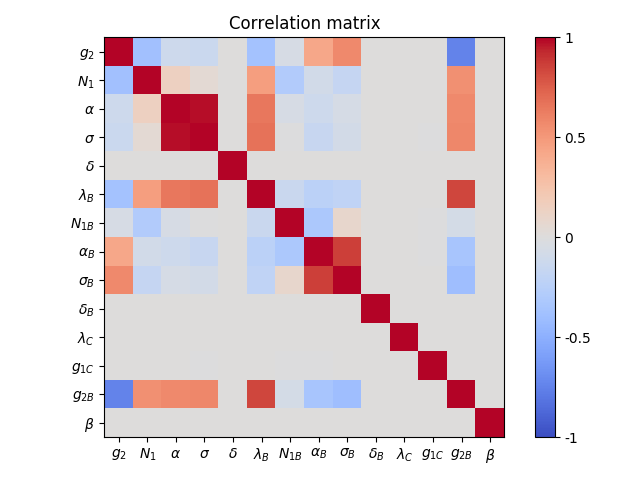
\includegraphics{pngplots/CorrelationMatrix.png}
\caption{Fitted parameter correlation matrix}
\end{figure}

\hypertarget{fit-properties}{%
\subsection{Fit properties}\label{fit-properties}}

\begin{figure}
\centering
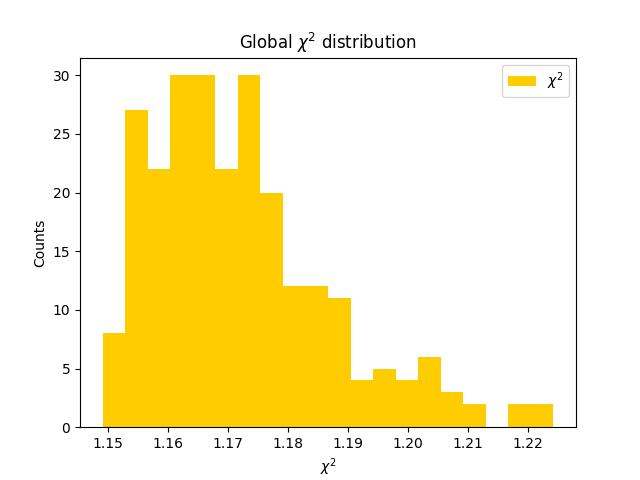
\includegraphics{pngplots/Globalchi2.png}
\caption{Global \(\chi^2\) distribution}
\end{figure}

\begin{figure}
\centering
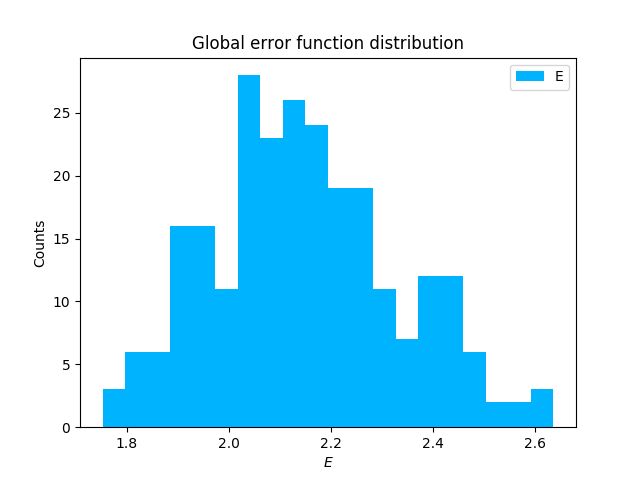
\includegraphics{pngplots/GlobalErrorFunction.png}
\caption{Global error function distribution}
\end{figure}

\begin{figure}
\centering
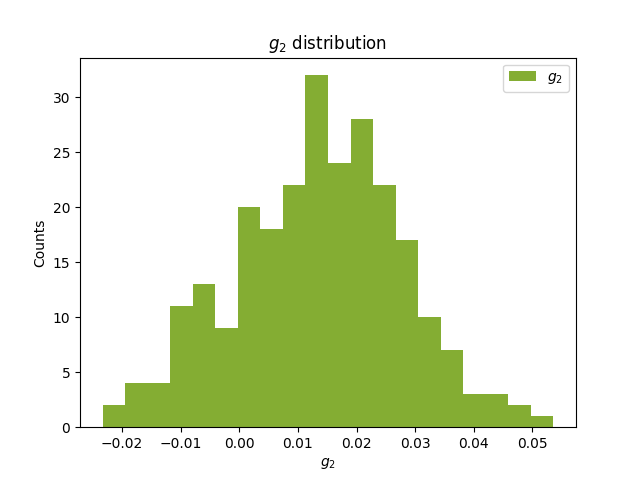
\includegraphics{pngplots/param0.png}
\caption{\(g_2\) distribution}
\end{figure}

\begin{figure}
\centering
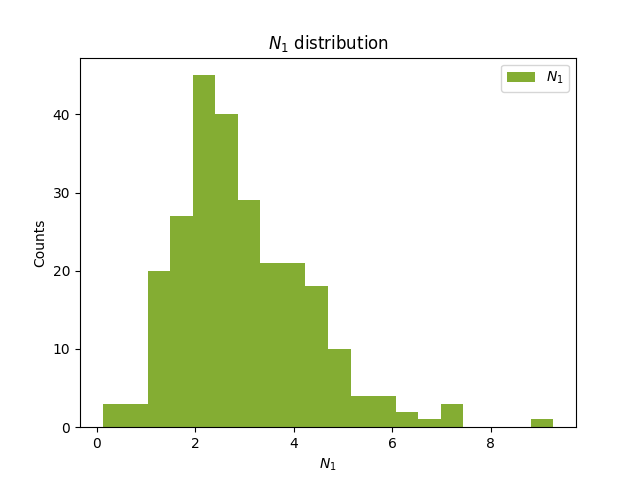
\includegraphics{pngplots/param1.png}
\caption{\(N_1\) distribution}
\end{figure}

\begin{figure}
\centering
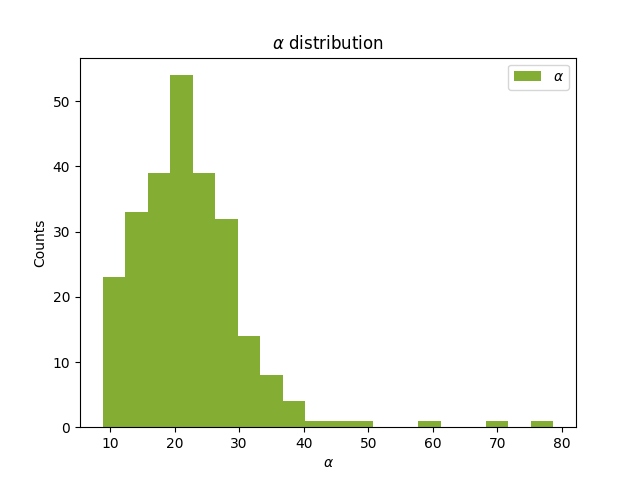
\includegraphics{pngplots/param2.png}
\caption{\(\alpha\) distribution}
\end{figure}

\begin{figure}
\centering
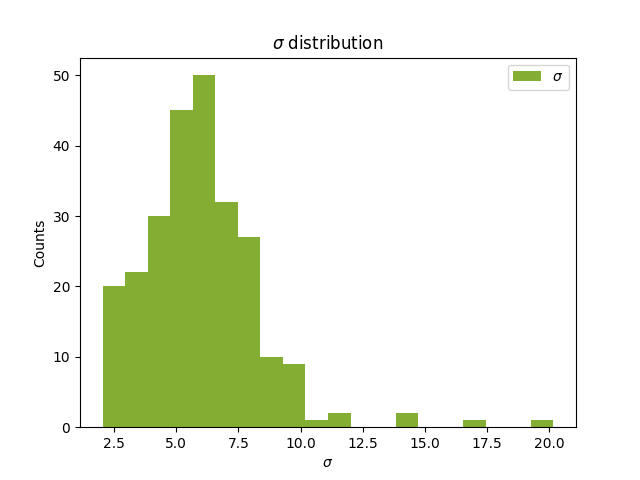
\includegraphics{pngplots/param3.png}
\caption{\(\sigma\) distribution}
\end{figure}

\begin{figure}
\centering
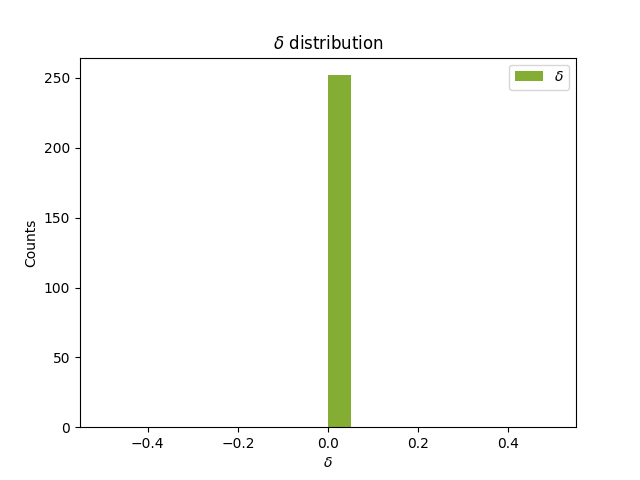
\includegraphics{pngplots/param4.png}
\caption{\(\delta\) distribution}
\end{figure}

\begin{figure}
\centering
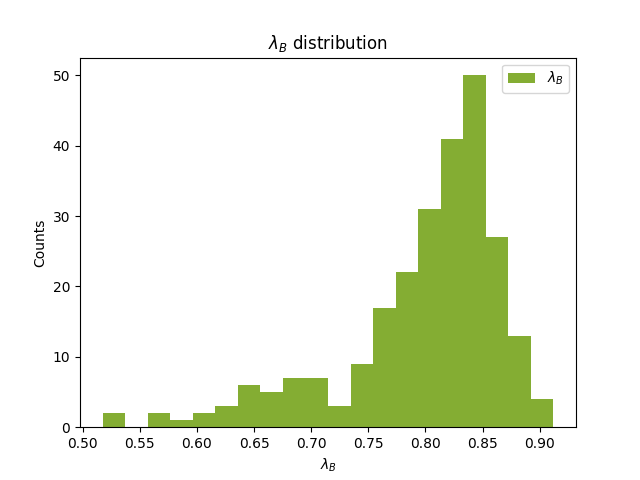
\includegraphics{pngplots/param5.png}
\caption{\(\lambda_B\) distribution}
\end{figure}

\begin{figure}
\centering
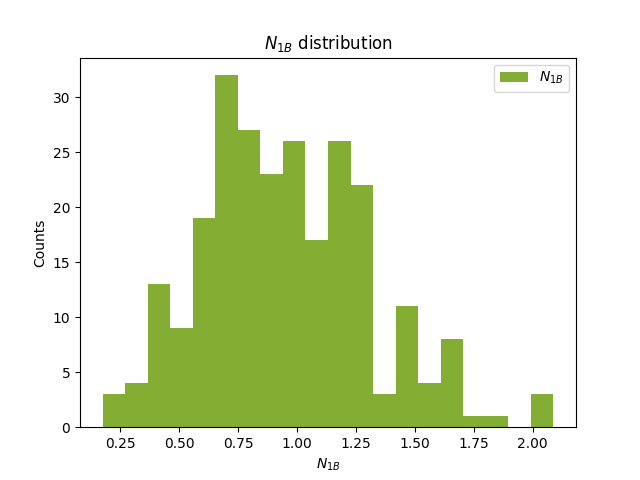
\includegraphics{pngplots/param6.png}
\caption{\(N_{1B}\) distribution}
\end{figure}

\begin{figure}
\centering
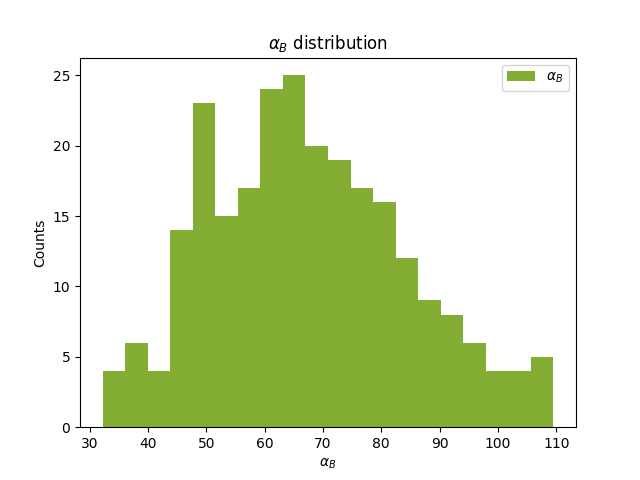
\includegraphics{pngplots/param7.png}
\caption{\(\alpha_B\) distribution}
\end{figure}

\begin{figure}
\centering
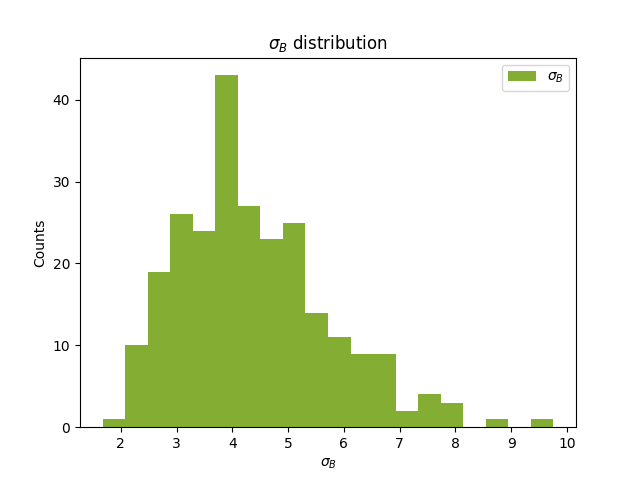
\includegraphics{pngplots/param8.png}
\caption{\(\sigma_B\) distribution}
\end{figure}

\begin{figure}
\centering
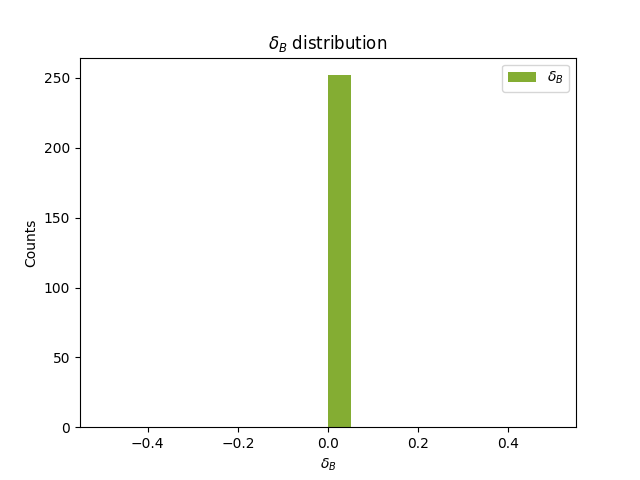
\includegraphics{pngplots/param9.png}
\caption{\(\delta_B\) distribution}
\end{figure}

\begin{figure}
\centering
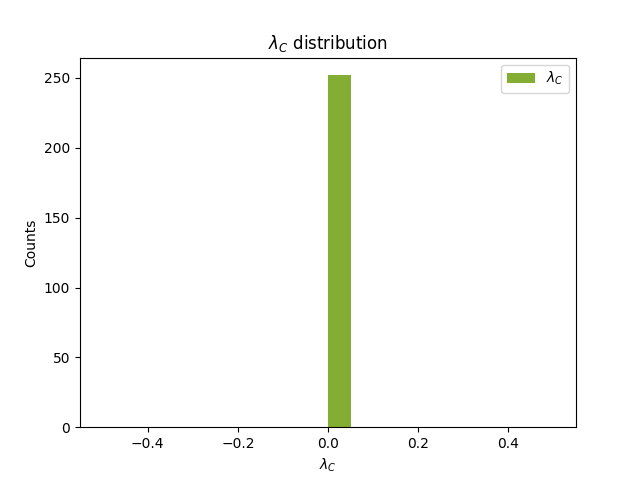
\includegraphics{pngplots/param10.png}
\caption{\(\lambda_C\) distribution}
\end{figure}

\begin{figure}
\centering
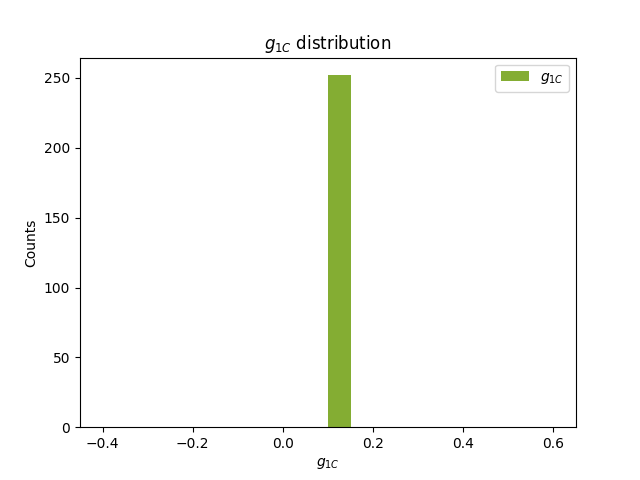
\includegraphics{pngplots/param11.png}
\caption{\(g_{1C}\) distribution}
\end{figure}

\begin{figure}
\centering
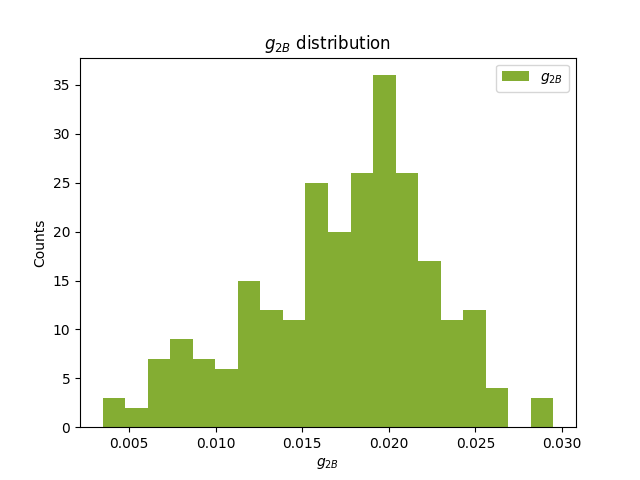
\includegraphics{pngplots/param12.png}
\caption{\(g_{2B}\) distribution}
\end{figure}

\begin{figure}
\centering
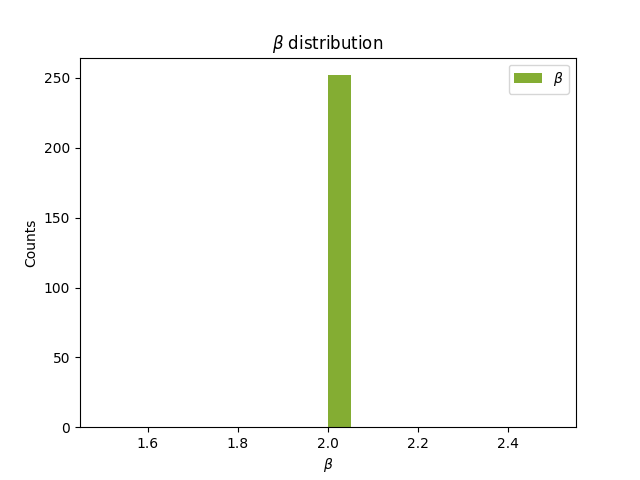
\includegraphics{pngplots/param13.png}
\caption{\(\beta\) distribution}
\end{figure}

\hypertarget{table-of-chi2s}{%
\subsection{\texorpdfstring{Table of
\(\chi^2\)'s}{Table of \textbackslash chi\^{}2's}}\label{table-of-chi2s}}

Central-replica \(\chi^2\)'s:

\begin{longtable}[]{@{}ccccc@{}}
\toprule
Experiment & Number of points & \(\chi_{D}^2\) & \(\chi_{\lambda}^2\) &
\(\chi^2\)\tabularnewline
\midrule
\endhead
E605\_Q\_7\_8 & 7 & 0.6145 & 0.0001 & 0.6146\tabularnewline
E605\_Q\_8\_9 & 8 & 1.5439 & 0.0004 & 1.5443\tabularnewline
E605\_Q\_10.5\_11.5 & 10 & 0.4725 & 0.2358 & 0.7083\tabularnewline
E288\_200\_Q\_4\_5 & 4 & 0.7716 & 0.9346 & 1.7062\tabularnewline
E288\_200\_Q\_5\_6 & 5 & 1.8219 & 0.2288 & 2.0507\tabularnewline
E288\_200\_Q\_6\_7 & 6 & 0.4223 & 0.0894 & 0.5117\tabularnewline
E288\_200\_Q\_7\_8 & 7 & 0.5384 & 0.0011 & 0.5395\tabularnewline
E288\_200\_Q\_8\_9 & 8 & 0.5815 & 0.0459 & 0.6274\tabularnewline
E288\_300\_Q\_4\_5 & 4 & 0.5827 & 0.4184 & 1.0011\tabularnewline
E288\_300\_Q\_5\_6 & 5 & 0.8974 & 0.1179 & 1.0153\tabularnewline
E288\_300\_Q\_6\_7 & 6 & 0.5684 & 0.0391 & 0.6075\tabularnewline
E288\_300\_Q\_7\_8 & 7 & 0.1675 & 0.0228 & 0.1903\tabularnewline
E288\_300\_Q\_8\_9 & 8 & 0.4581 & 0.0078 & 0.4659\tabularnewline
E288\_400\_Q\_5\_6 & 5 & 0.3296 & 0.0004 & 0.33\tabularnewline
E288\_400\_Q\_6\_7 & 6 & 0.0903 & 0.0033 & 0.0936\tabularnewline
E288\_400\_Q\_7\_8 & 7 & 0.0299 & 0.0129 & 0.0428\tabularnewline
E288\_400\_Q\_8\_9 & 8 & 0.468 & 0.0238 & 0.4918\tabularnewline
E288\_400\_Q\_11\_12 & 11 & 0.4963 & 0.0595 & 0.5558\tabularnewline
E288\_400\_Q\_12\_13 & 12 & 0.4711 & 0.0631 & 0.5342\tabularnewline
E288\_400\_Q\_13\_14 & 12 & 0.5142 & 0.1115 & 0.6258\tabularnewline
STAR\_510 & 7 & 0.9242 & 0.0358 & 0.96\tabularnewline
CDF\_RunI & 25 & 0.5303 & 0.0574 & 0.5878\tabularnewline
CDF\_RunII & 26 & 0.8489 & 0.0024 & 0.8512\tabularnewline
D0\_RunI & 12 & 0.6072 & 0.0447 & 0.6518\tabularnewline
D0\_RunII & 5 & 0.9414 & 0.5915 & 1.5329\tabularnewline
D0\_RunIImu & 3 & 3.0096 & 0.0215 & 3.0312\tabularnewline
LHCb\_7TeV & 7 & 1.1171 & 0.1469 & 1.2639\tabularnewline
LHCb\_8TeV & 7 & 0.5648 & 0.0948 & 0.6596\tabularnewline
LHCb\_13TeV & 7 & 0.918 & 0.0243 & 0.9423\tabularnewline
CMS\_7TeV & 4 & 2.114 & 0 & 2.114\tabularnewline
CMS\_8TeV & 4 & 1.3572 & 0.009 & 1.3661\tabularnewline
ATLAS\_7TeV\_y\_0\_1 & 6 & 2.3745 & 0.0255 & 2.4\tabularnewline
ATLAS\_7TeV\_y\_1\_2 & 6 & 4.0729 & 1.0428 & 5.1157\tabularnewline
ATLAS\_7TeV\_y\_2\_2.4 & 6 & 3.4912 & 0.3862 & 3.8774\tabularnewline
ATLAS\_8TeV\_y\_0\_0.4 & 6 & 2.0616 & 0.149 & 2.2106\tabularnewline
ATLAS\_8TeV\_y\_0.4\_0.8 & 6 & 2.2188 & 0.3225 & 2.5414\tabularnewline
ATLAS\_8TeV\_y\_0.8\_1.2 & 6 & 1.504 & 0.2847 & 1.7887\tabularnewline
ATLAS\_8TeV\_y\_1.2\_1.6 & 6 & 1.9611 & 0.4008 & 2.3619\tabularnewline
ATLAS\_8TeV\_y\_1.6\_2 & 6 & 3.1533 & 0.8328 & 3.9861\tabularnewline
ATLAS\_8TeV\_y\_2\_2.4 & 6 & 0.704 & 0.011 & 0.7149\tabularnewline
ATLAS\_8TeV\_Q\_46\_66 & 4 & 2.1141 & 0.783 & 2.8971\tabularnewline
ATLAS\_8TeV\_Q\_116\_150 & 8 & 0.502 & 0.004 & 0.506\tabularnewline
Total & 319 & - & - & 1.1432\tabularnewline
\bottomrule
\end{longtable}

Mean-replica \(\chi^2\)'s:

\begin{longtable}[]{@{}ccccc@{}}
\toprule
Experiment & Number of points & \(\chi_{D}^2\) & \(\chi_{\lambda}^2\) &
\(\chi^2\)\tabularnewline
\midrule
\endhead
E605\_Q\_7\_8 & 7 & 0.5137 & 0.0001 & 0.5138\tabularnewline
E605\_Q\_8\_9 & 8 & 1.409 & 0.0012 & 1.4103\tabularnewline
E605\_Q\_10.5\_11.5 & 10 & 0.424 & 0.1295 & 0.5536\tabularnewline
E288\_200\_Q\_4\_5 & 4 & 0.386 & 0.4599 & 0.8458\tabularnewline
E288\_200\_Q\_5\_6 & 5 & 1.2471 & 0.1259 & 1.373\tabularnewline
E288\_200\_Q\_6\_7 & 6 & 0.345 & 0.051 & 0.396\tabularnewline
E288\_200\_Q\_7\_8 & 7 & 0.6056 & 0.0018 & 0.6074\tabularnewline
E288\_200\_Q\_8\_9 & 8 & 0.8596 & 0.0289 & 0.8886\tabularnewline
E288\_300\_Q\_4\_5 & 4 & 0.391 & 0.2572 & 0.6481\tabularnewline
E288\_300\_Q\_5\_6 & 5 & 0.7401 & 0.0568 & 0.797\tabularnewline
E288\_300\_Q\_6\_7 & 6 & 0.5034 & 0.012 & 0.5155\tabularnewline
E288\_300\_Q\_7\_8 & 7 & 0.1448 & 0.0059 & 0.1507\tabularnewline
E288\_300\_Q\_8\_9 & 8 & 0.4225 & 0.0036 & 0.4261\tabularnewline
E288\_400\_Q\_5\_6 & 5 & 0.4797 & 0.0109 & 0.4906\tabularnewline
E288\_400\_Q\_6\_7 & 6 & 0.1138 & 0.0295 & 0.1433\tabularnewline
E288\_400\_Q\_7\_8 & 7 & 0.0496 & 0.0453 & 0.0949\tabularnewline
E288\_400\_Q\_8\_9 & 8 & 0.6887 & 0.0507 & 0.7394\tabularnewline
E288\_400\_Q\_11\_12 & 11 & 0.754 & 0.0845 & 0.8385\tabularnewline
E288\_400\_Q\_12\_13 & 12 & 0.8261 & 0.0652 & 0.8914\tabularnewline
E288\_400\_Q\_13\_14 & 12 & 1.1479 & 0.071 & 1.2189\tabularnewline
STAR\_510 & 7 & 0.8142 & 0.0667 & 0.8809\tabularnewline
CDF\_RunI & 25 & 0.4778 & 0.0608 & 0.5386\tabularnewline
CDF\_RunII & 26 & 0.824 & 0.0006 & 0.8246\tabularnewline
D0\_RunI & 12 & 0.6146 & 0.0395 & 0.6541\tabularnewline
D0\_RunII & 5 & 0.9719 & 0.5849 & 1.5569\tabularnewline
D0\_RunIImu & 3 & 3.39 & 0.0368 & 3.4267\tabularnewline
LHCb\_7TeV & 7 & 0.9889 & 0.1665 & 1.1554\tabularnewline
LHCb\_8TeV & 7 & 0.5721 & 0.1093 & 0.6814\tabularnewline
LHCb\_13TeV & 7 & 0.9156 & 0.0264 & 0.9421\tabularnewline
CMS\_7TeV & 4 & 2.1031 & 0 & 2.1031\tabularnewline
CMS\_8TeV & 4 & 1.3807 & 0.008 & 1.3887\tabularnewline
ATLAS\_7TeV\_y\_0\_1 & 6 & 2.407 & 0.0262 & 2.4332\tabularnewline
ATLAS\_7TeV\_y\_1\_2 & 6 & 4.0104 & 1.042 & 5.0525\tabularnewline
ATLAS\_7TeV\_y\_2\_2.4 & 6 & 3.3577 & 0.3876 & 3.7453\tabularnewline
ATLAS\_8TeV\_y\_0\_0.4 & 6 & 2.1623 & 0.1378 & 2.3001\tabularnewline
ATLAS\_8TeV\_y\_0.4\_0.8 & 6 & 2.1945 & 0.299 & 2.4935\tabularnewline
ATLAS\_8TeV\_y\_0.8\_1.2 & 6 & 1.4912 & 0.2791 & 1.7704\tabularnewline
ATLAS\_8TeV\_y\_1.2\_1.6 & 6 & 1.9356 & 0.3985 & 2.3341\tabularnewline
ATLAS\_8TeV\_y\_1.6\_2 & 6 & 3.1664 & 0.8248 & 3.9912\tabularnewline
ATLAS\_8TeV\_y\_2\_2.4 & 6 & 0.5992 & 0.0138 & 0.6131\tabularnewline
ATLAS\_8TeV\_Q\_46\_66 & 4 & 2.2328 & 0.739 & 2.9718\tabularnewline
ATLAS\_8TeV\_Q\_116\_150 & 8 & 0.499 & 0.0036 & 0.5026\tabularnewline
Total & 319 & - & - & 1.1526\tabularnewline
\bottomrule
\end{longtable}

Average-over-replicas \(\chi^2\)'s:

\begin{longtable}[]{@{}ccccc@{}}
\toprule
Experiment & Number of points & \(\chi_{D}^2\) & \(\chi_{\lambda}^2\) &
\(\chi^2\)\tabularnewline
\midrule
\endhead
E605\_Q\_7\_8 & 7 & 0.4879 \(\pm\) 0.2025 & 0.1351 \(\pm\) 0.1793 &
0.623 \(\pm\) 0.0997\tabularnewline
E605\_Q\_8\_9 & 8 & 1.406 \(\pm\) 0.2955 & 0.0999 \(\pm\) 0.1419 &
1.5058 \(\pm\) 0.2511\tabularnewline
E605\_Q\_10.5\_11.5 & 10 & 0.4437 \(\pm\) 0.3709 & 0.2914 \(\pm\) 0.3353
& 0.7351 \(\pm\) 0.1275\tabularnewline
E288\_200\_Q\_4\_5 & 4 & 0.51 \(\pm\) 1.5998 & 1.3084 \(\pm\) 1.5115 &
1.8183 \(\pm\) 0.354\tabularnewline
E288\_200\_Q\_5\_6 & 5 & 1.571 \(\pm\) 0.8118 & 0.5191 \(\pm\) 0.7237 &
2.0902 \(\pm\) 0.2751\tabularnewline
E288\_200\_Q\_6\_7 & 6 & 0.2122 \(\pm\) 0.4418 & 0.3274 \(\pm\) 0.4161 &
0.5396 \(\pm\) 0.1401\tabularnewline
E288\_200\_Q\_7\_8 & 7 & 0.3954 \(\pm\) 0.2709 & 0.1494 \(\pm\) 0.1976 &
0.5448 \(\pm\) 0.2027\tabularnewline
E288\_200\_Q\_8\_9 & 8 & 0.4798 \(\pm\) 0.1747 & 0.1566 \(\pm\) 0.169 &
0.6364 \(\pm\) 0.0818\tabularnewline
E288\_300\_Q\_4\_5 & 4 & 0.3261 \(\pm\) 1.0797 & 0.774 \(\pm\) 1.0086 &
1.1001 \(\pm\) 0.2661\tabularnewline
E288\_300\_Q\_5\_6 & 5 & 0.7075 \(\pm\) 0.51 & 0.3592 \(\pm\) 0.46 &
1.0667 \(\pm\) 0.1646\tabularnewline
E288\_300\_Q\_6\_7 & 6 & 0.4065 \(\pm\) 0.3454 & 0.2189 \(\pm\) 0.2904 &
0.6254 \(\pm\) 0.1623\tabularnewline
E288\_300\_Q\_7\_8 & 7 & 0.026 \(\pm\) 0.255 & 0.1759 \(\pm\) 0.2374 &
0.2019 \(\pm\) 0.0712\tabularnewline
E288\_300\_Q\_8\_9 & 8 & 0.3655 \(\pm\) 0.209 & 0.1303 \(\pm\) 0.2001 &
0.4959 \(\pm\) 0.0998\tabularnewline
E288\_400\_Q\_5\_6 & 5 & 0.2088 \(\pm\) 0.275 & 0.1869 \(\pm\) 0.2354 &
0.3957 \(\pm\) 0.1311\tabularnewline
E288\_400\_Q\_6\_7 & 6 & 0.0074 \(\pm\) 0.1904 & 0.1294 \(\pm\) 0.1869 &
0.1367 \(\pm\) 0.0518\tabularnewline
E288\_400\_Q\_7\_8 & 7 & -0.047 \(\pm\) 0.1809 & 0.1331 \(\pm\) 0.175 &
0.0861 \(\pm\) 0.0577\tabularnewline
E288\_400\_Q\_8\_9 & 8 & 0.4002 \(\pm\) 0.1977 & 0.1271 \(\pm\) 0.1719 &
0.5272 \(\pm\) 0.1006\tabularnewline
E288\_400\_Q\_11\_12 & 11 & 0.494 \(\pm\) 0.2296 & 0.1136 \(\pm\) 0.1357
& 0.6077 \(\pm\) 0.1771\tabularnewline
E288\_400\_Q\_12\_13 & 12 & 0.456 \(\pm\) 0.1382 & 0.1231 \(\pm\) 0.1355
& 0.5792 \(\pm\) 0.0475\tabularnewline
E288\_400\_Q\_13\_14 & 12 & 0.502 \(\pm\) 0.1393 & 0.1424 \(\pm\) 0.1304
& 0.6444 \(\pm\) 0.0595\tabularnewline
STAR\_510 & 7 & 0.8411 \(\pm\) 0.2163 & 0.1397 \(\pm\) 0.2116 & 0.9808
\(\pm\) 0.0539\tabularnewline
CDF\_RunI & 25 & 0.4938 \(\pm\) 0.1171 & 0.1002 \(\pm\) 0.1162 & 0.594
\(\pm\) 0.0163\tabularnewline
CDF\_RunII & 26 & 0.8427 \(\pm\) 0.0873 & 0.0428 \(\pm\) 0.0534 & 0.8855
\(\pm\) 0.0699\tabularnewline
D0\_RunI & 12 & 0.5478 \(\pm\) 0.1471 & 0.1063 \(\pm\) 0.1415 & 0.6541
\(\pm\) 0.0358\tabularnewline
D0\_RunII & 5 & 0.8052 \(\pm\) 0.7828 & 0.7652 \(\pm\) 0.7682 & 1.5704
\(\pm\) 0.2595\tabularnewline
D0\_RunIImu & 3 & 2.5219 \(\pm\) 0.7733 & 0.5047 \(\pm\) 0.555 & 3.0266
\(\pm\) 0.555\tabularnewline
LHCb\_7TeV & 7 & 0.9494 \(\pm\) 0.3224 & 0.3363 \(\pm\) 0.3142 & 1.2857
\(\pm\) 0.0576\tabularnewline
LHCb\_8TeV & 7 & 0.492 \(\pm\) 0.3581 & 0.2254 \(\pm\) 0.3013 & 0.7175
\(\pm\) 0.1816\tabularnewline
LHCb\_13TeV & 7 & 0.8811 \(\pm\) 0.2042 & 0.1111 \(\pm\) 0.1738 & 0.9922
\(\pm\) 0.1332\tabularnewline
CMS\_7TeV & 4 & 2.118 \(\pm\) 0.013 & 0.0 \(\pm\) 0.0 & 2.118 \(\pm\)
0.013\tabularnewline
CMS\_8TeV & 4 & 1.2997 \(\pm\) 0.1153 & 0.0659 \(\pm\) 0.0987 & 1.3655
\(\pm\) 0.0564\tabularnewline
ATLAS\_7TeV\_y\_0\_1 & 6 & 2.3364 \(\pm\) 0.2619 & 0.0999 \(\pm\) 0.1479
& 2.4362 \(\pm\) 0.2269\tabularnewline
ATLAS\_7TeV\_y\_1\_2 & 6 & 4.1293 \(\pm\) 0.4726 & 1.0555 \(\pm\) 0.4477
& 5.1848 \(\pm\) 0.1239\tabularnewline
ATLAS\_7TeV\_y\_2\_2.4 & 6 & 3.4956 \(\pm\) 0.194 & 0.4102 \(\pm\)
0.1653 & 3.9058 \(\pm\) 0.107\tabularnewline
ATLAS\_8TeV\_y\_0\_0.4 & 6 & 2.029 \(\pm\) 0.2625 & 0.2185 \(\pm\)
0.2075 & 2.2475 \(\pm\) 0.2038\tabularnewline
ATLAS\_8TeV\_y\_0.4\_0.8 & 6 & 2.2027 \(\pm\) 0.3391 & 0.3877 \(\pm\)
0.3204 & 2.5904 \(\pm\) 0.1032\tabularnewline
ATLAS\_8TeV\_y\_0.8\_1.2 & 6 & 1.4878 \(\pm\) 0.2072 & 0.3305 \(\pm\)
0.2036 & 1.8182 \(\pm\) 0.0603\tabularnewline
ATLAS\_8TeV\_y\_1.2\_1.6 & 6 & 1.9399 \(\pm\) 0.3127 & 0.4437 \(\pm\)
0.2907 & 2.3836 \(\pm\) 0.1219\tabularnewline
ATLAS\_8TeV\_y\_1.6\_2 & 6 & 3.1364 \(\pm\) 0.5551 & 0.9437 \(\pm\)
0.5319 & 4.0801 \(\pm\) 0.2352\tabularnewline
ATLAS\_8TeV\_y\_2\_2.4 & 6 & 0.6794 \(\pm\) 0.2202 & 0.0676 \(\pm\)
0.0908 & 0.747 \(\pm\) 0.2138\tabularnewline
ATLAS\_8TeV\_Q\_46\_66 & 4 & 1.9295 \(\pm\) 0.7599 & 0.9589 \(\pm\)
0.7467 & 2.8885 \(\pm\) 0.1032\tabularnewline
ATLAS\_8TeV\_Q\_116\_150 & 8 & 0.4081 \(\pm\) 0.1789 & 0.1039 \(\pm\)
0.1792 & 0.5119 \(\pm\) 0.016\tabularnewline
Total & 319 & - & - & 1.1721 \(\pm\) 0.015\tabularnewline
\bottomrule
\end{longtable}

\hypertarget{tmds-in-k_t-space}{%
\subsection{\texorpdfstring{TMDs in \(k_T\)
space}{TMDs in k\_T space}}\label{tmds-in-k_t-space}}

\begin{figure}
\centering
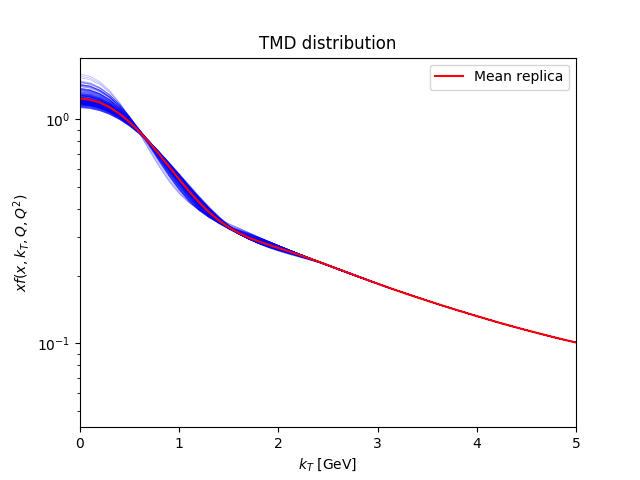
\includegraphics{pngplots/tmd_1_2_0.001.png}
\caption{TMD PDF of the \(d\) at \(Q = 2\) GeV and \(x = 0.001\)}
\end{figure}

\begin{figure}
\centering
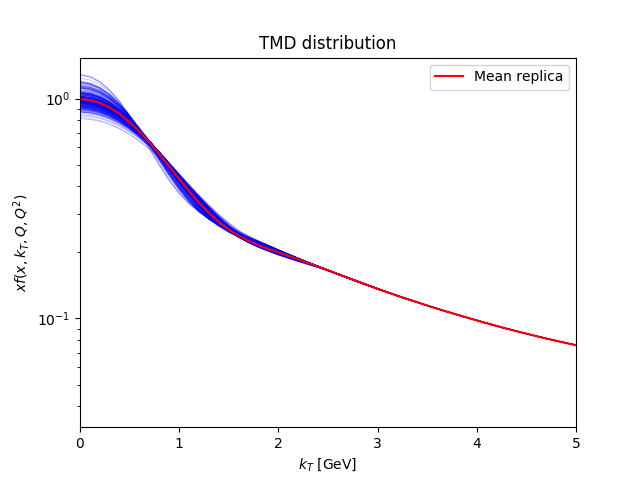
\includegraphics{pngplots/tmd_1_2_0.01.png}
\caption{TMD PDF of the \(d\) at \(Q = 2\) GeV and \(x = 0.01\)}
\end{figure}

\begin{figure}
\centering
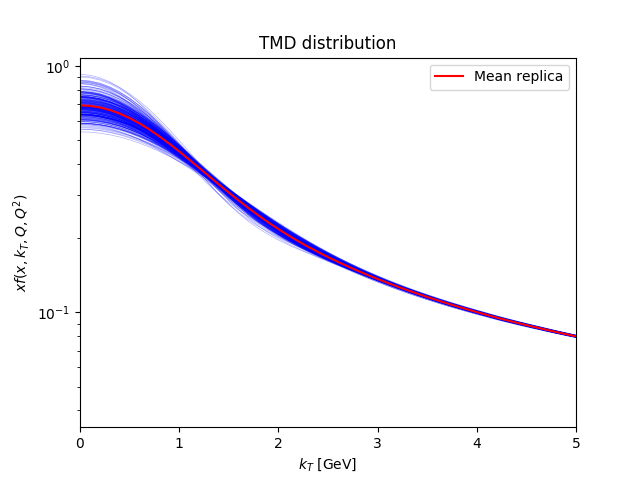
\includegraphics{pngplots/tmd_1_2_0.1.png}
\caption{TMD PDF of the \(d\) at \(Q = 2\) GeV and \(x = 0.1\)}
\end{figure}

\begin{figure}
\centering
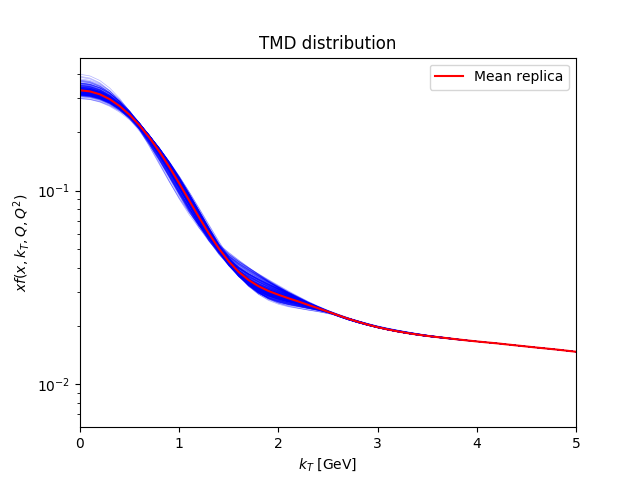
\includegraphics{pngplots/tmd_1_2_0.5.png}
\caption{TMD PDF of the \(d\) at \(Q = 2\) GeV and \(x = 0.5\)}
\end{figure}

\begin{figure}
\centering
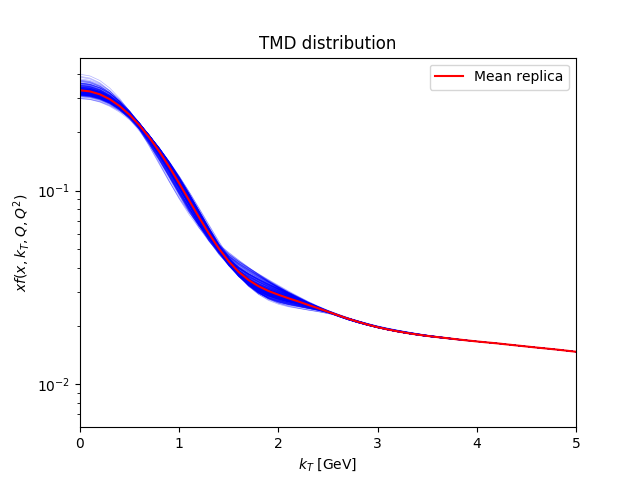
\includegraphics{pngplots/tmd_1_2_0.9.png}
\caption{TMD PDF of the \(d\) at \(Q = 2\) GeV and \(x = 0.9\)}
\end{figure}

\hypertarget{data-theory-comparison}{%
\subsection{Data-theory comparison}\label{data-theory-comparison}}

\begin{figure}
\centering
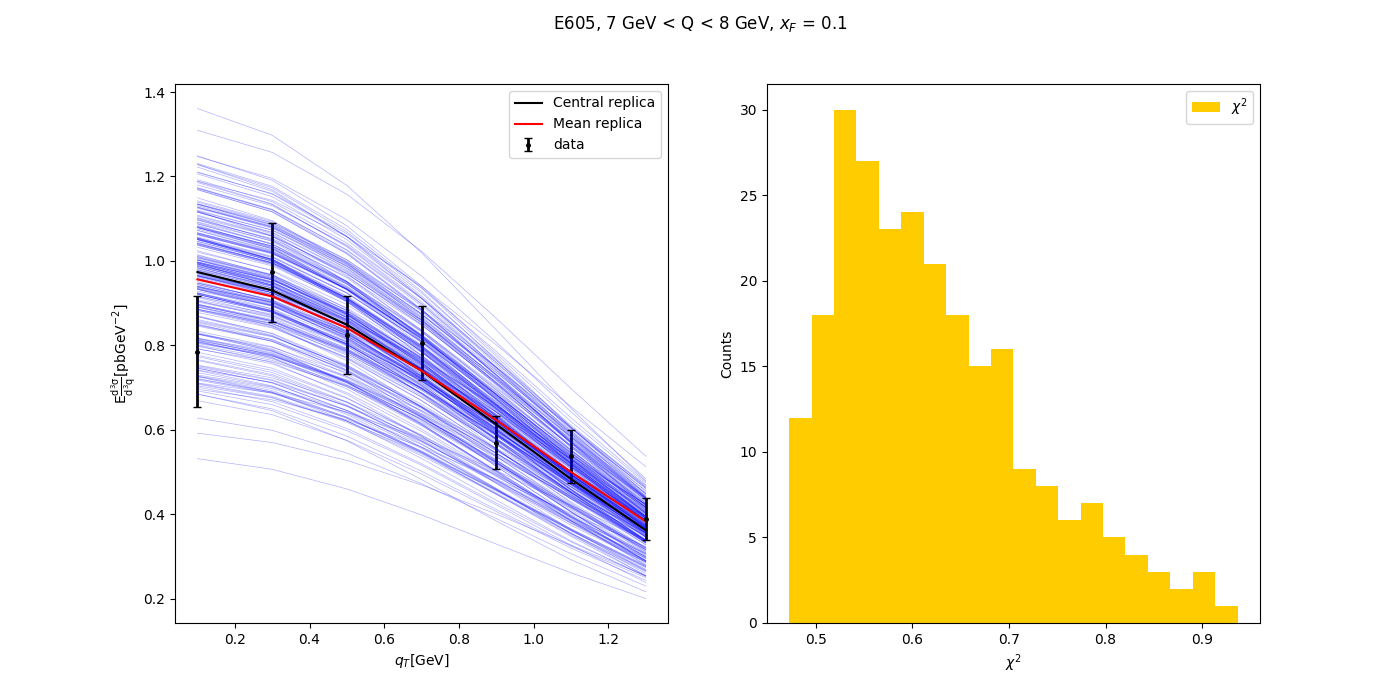
\includegraphics{pngplots/E605_Q_7_8.png}
\caption{E605\_Q\_7\_8 data-theory comparison}
\end{figure}

\begin{figure}
\centering
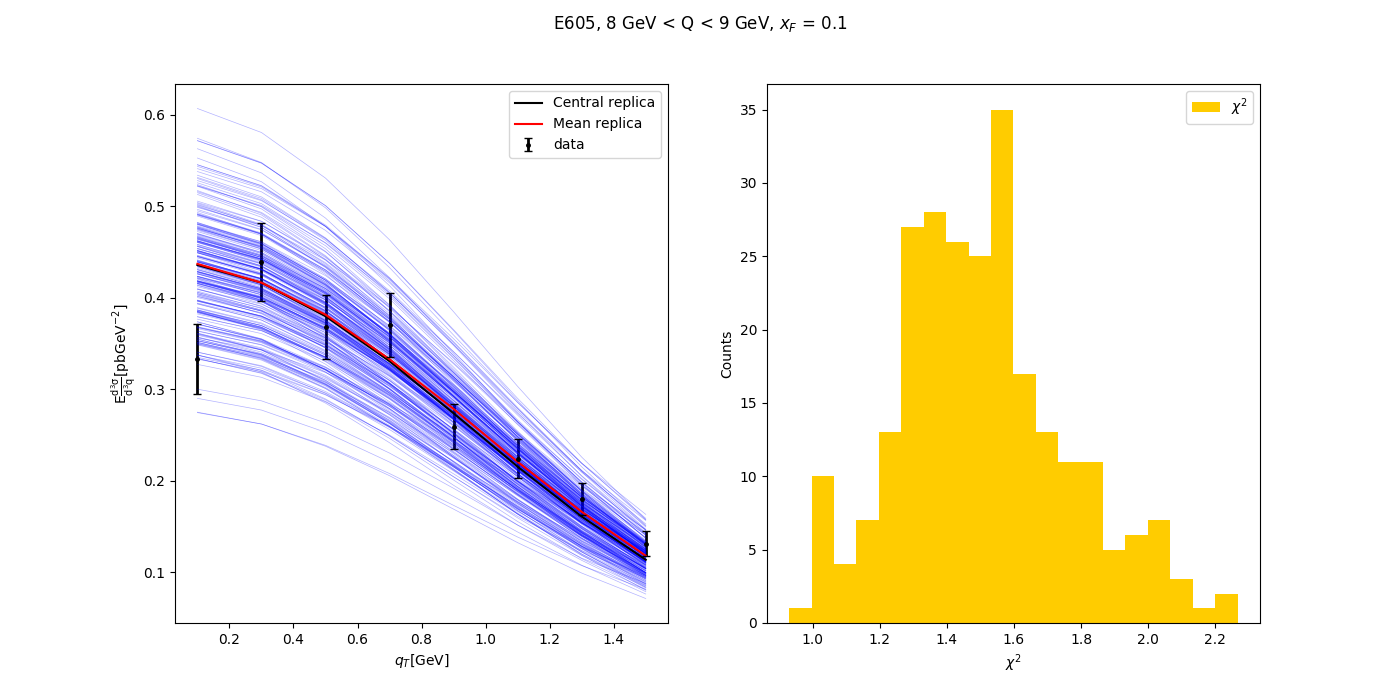
\includegraphics{pngplots/E605_Q_8_9.png}
\caption{E605\_Q\_8\_9 data-theory comparison}
\end{figure}

\begin{figure}
\centering
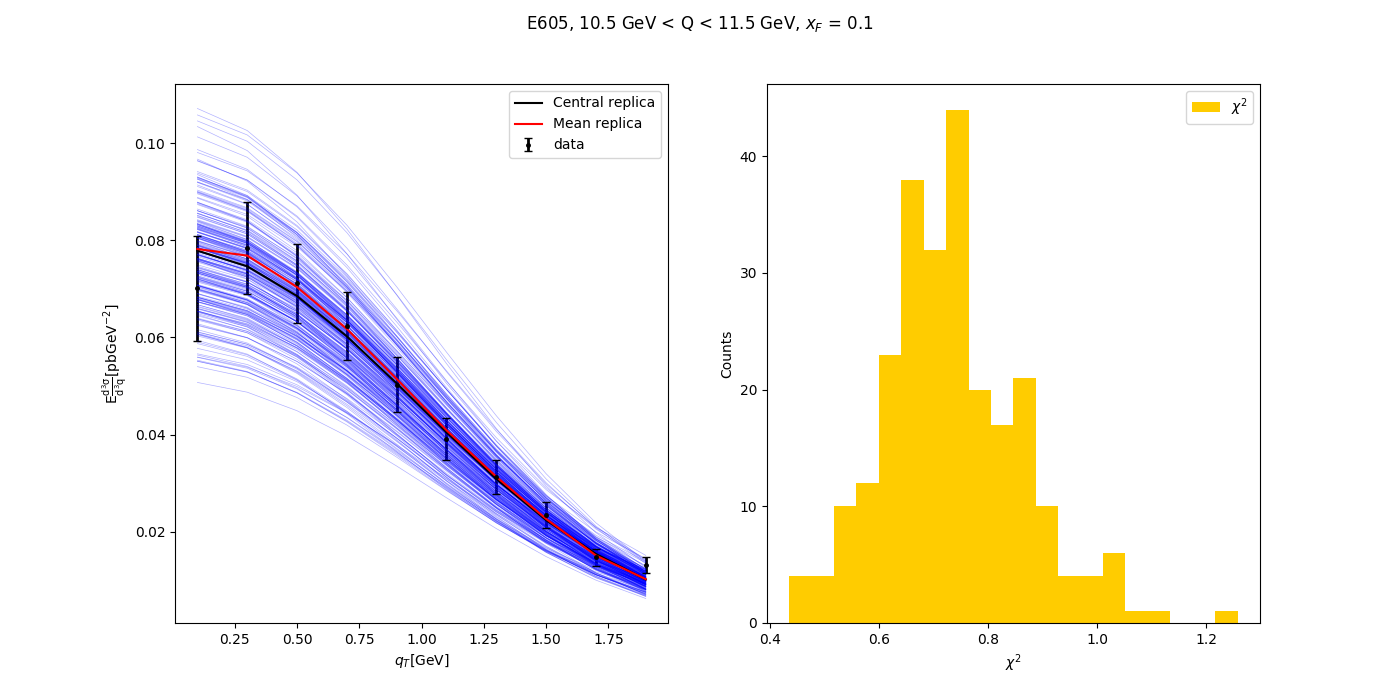
\includegraphics{pngplots/E605_Q_10.5_11.5.png}
\caption{E605\_Q\_10.5\_11.5 data-theory comparison}
\end{figure}

\begin{figure}
\centering
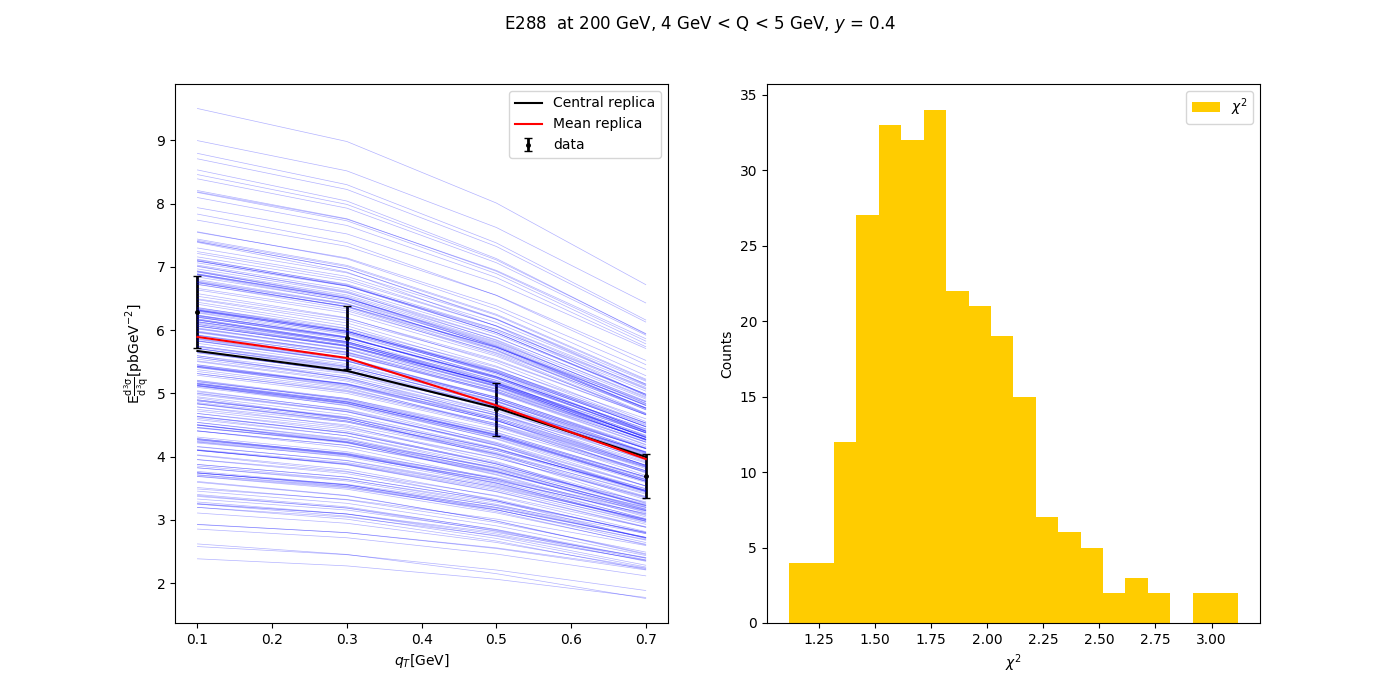
\includegraphics{pngplots/E288_200_Q_4_5.png}
\caption{E288\_200\_Q\_4\_5 data-theory comparison}
\end{figure}

\begin{figure}
\centering
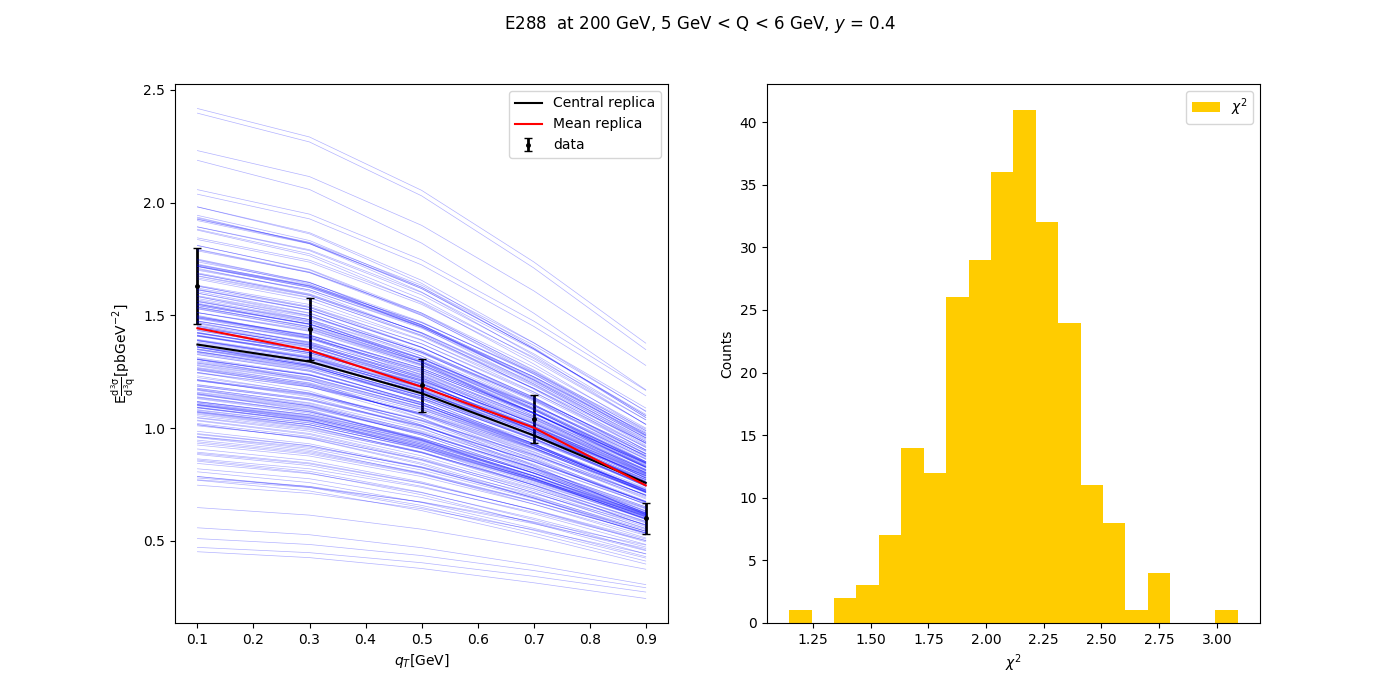
\includegraphics{pngplots/E288_200_Q_5_6.png}
\caption{E288\_200\_Q\_5\_6 data-theory comparison}
\end{figure}

\begin{figure}
\centering
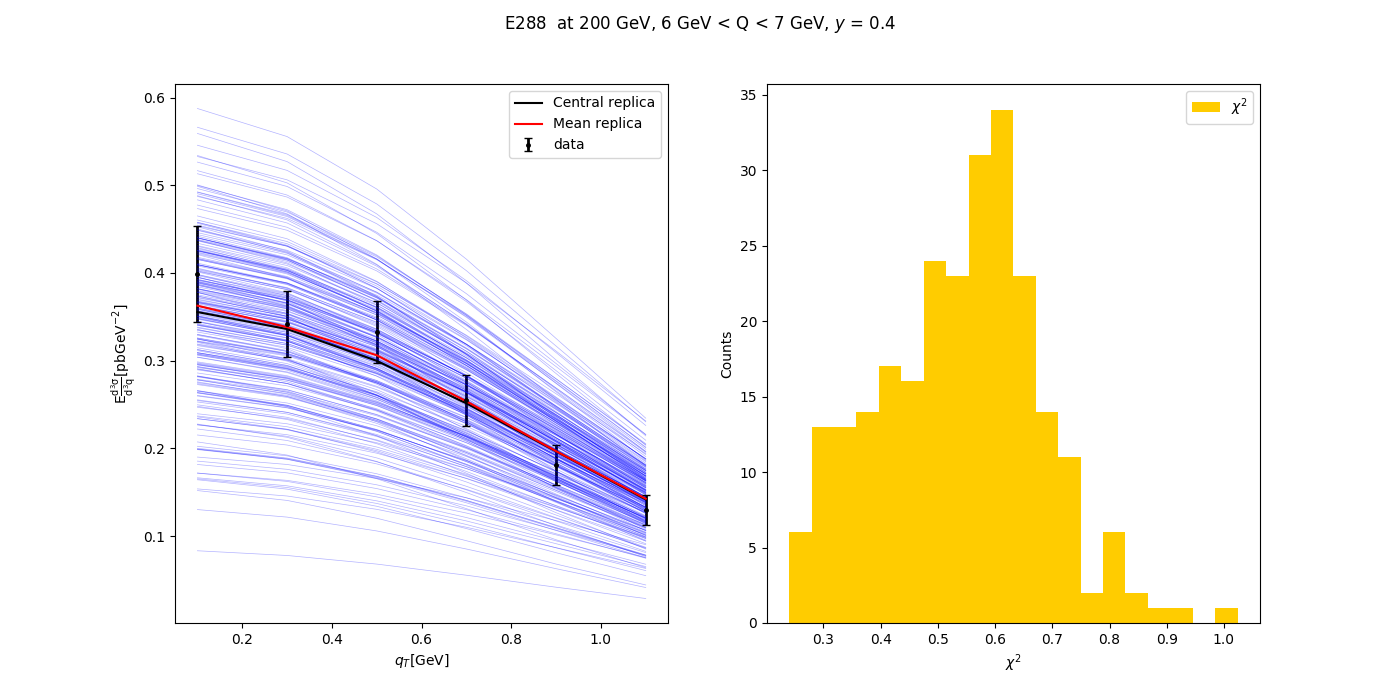
\includegraphics{pngplots/E288_200_Q_6_7.png}
\caption{E288\_200\_Q\_6\_7 data-theory comparison}
\end{figure}

\begin{figure}
\centering
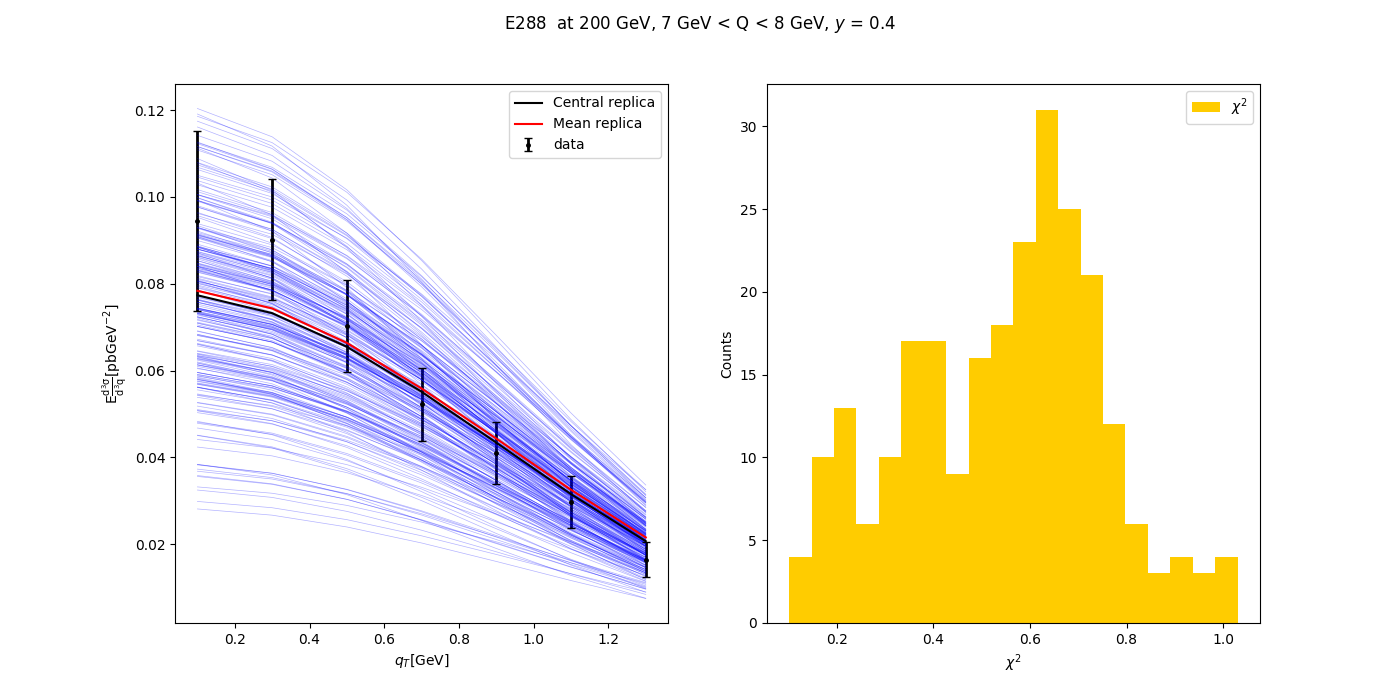
\includegraphics{pngplots/E288_200_Q_7_8.png}
\caption{E288\_200\_Q\_7\_8 data-theory comparison}
\end{figure}

\begin{figure}
\centering
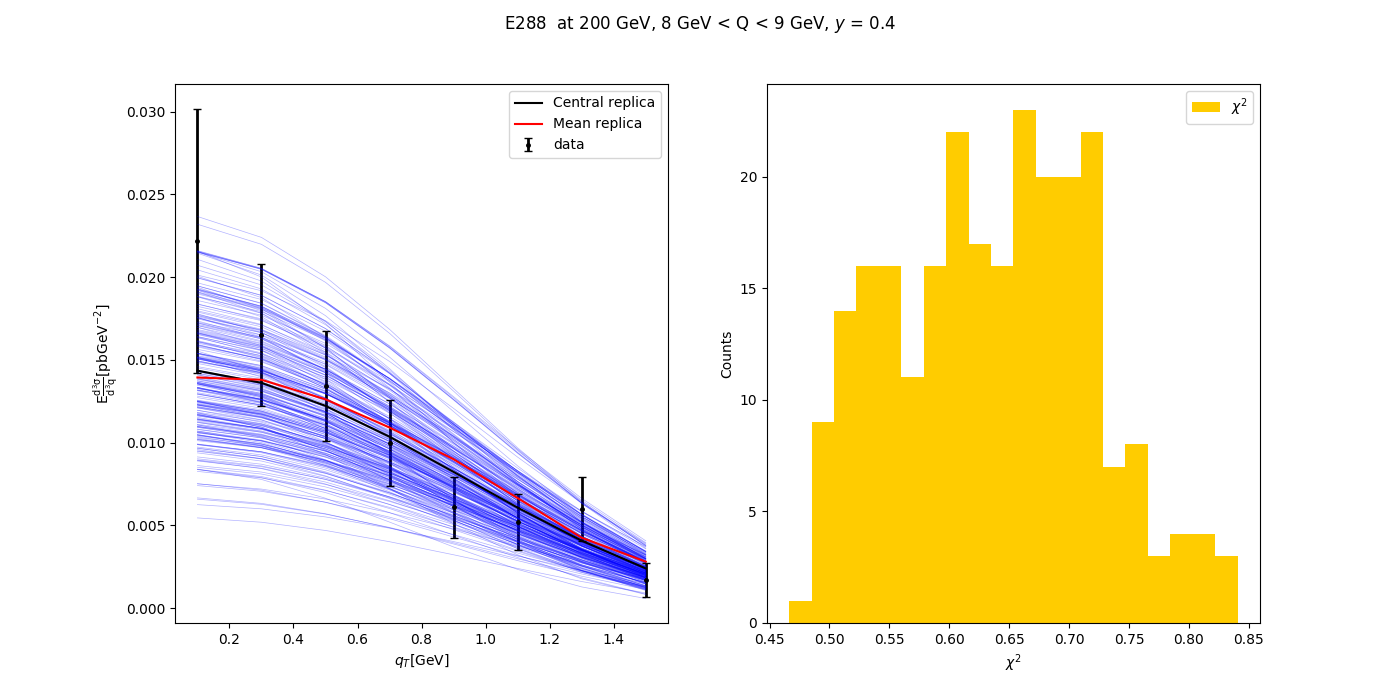
\includegraphics{pngplots/E288_200_Q_8_9.png}
\caption{E288\_200\_Q\_8\_9 data-theory comparison}
\end{figure}

\begin{figure}
\centering
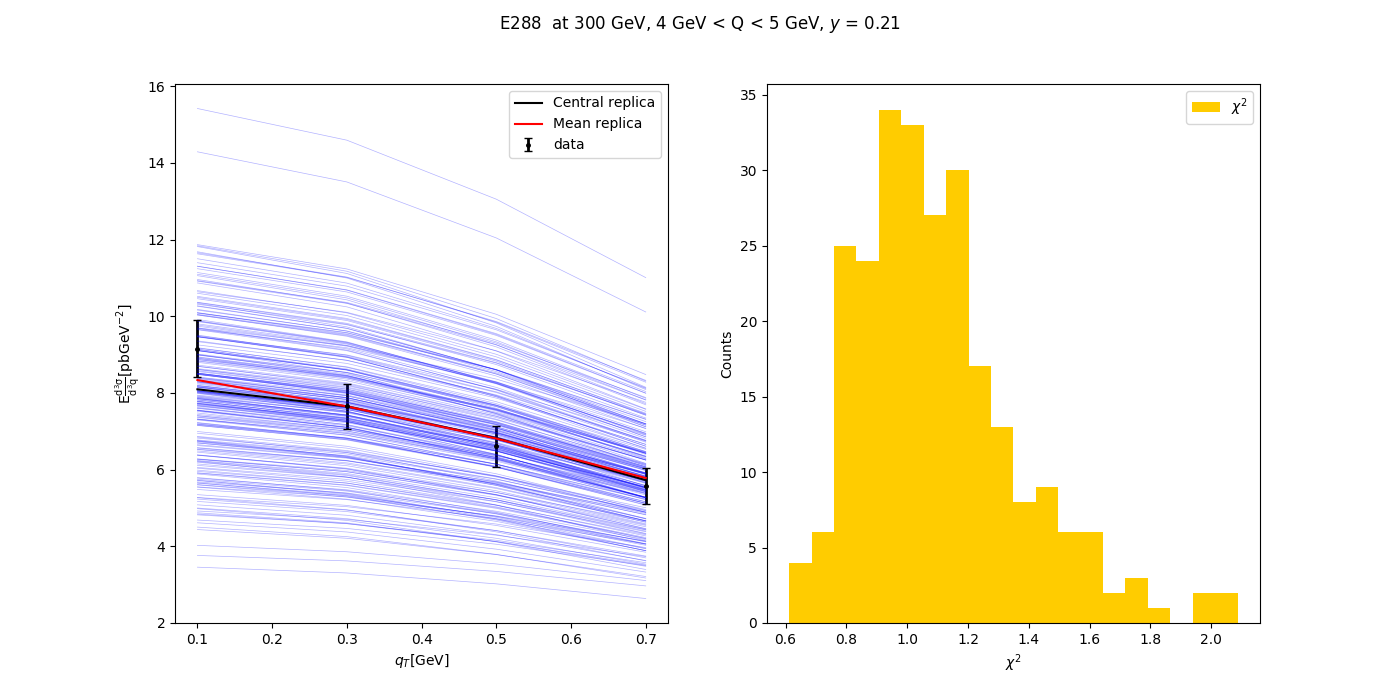
\includegraphics{pngplots/E288_300_Q_4_5.png}
\caption{E288\_300\_Q\_4\_5 data-theory comparison}
\end{figure}

\begin{figure}
\centering
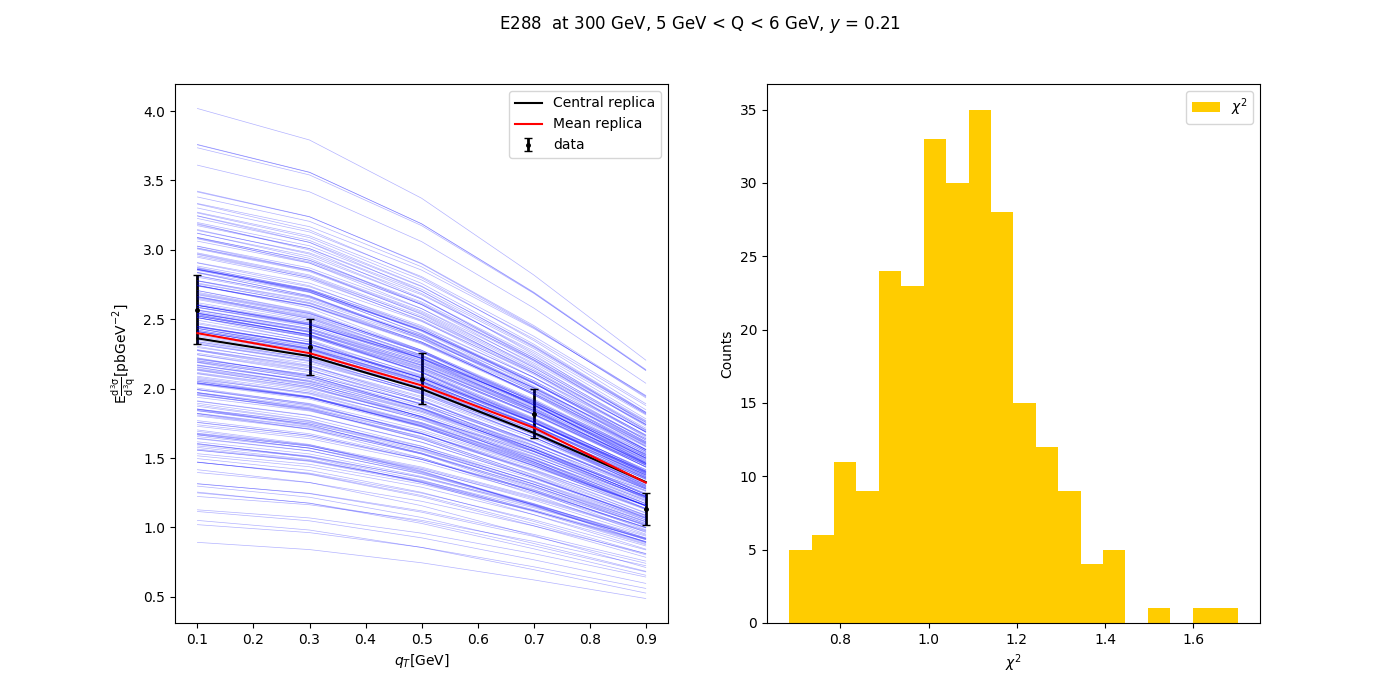
\includegraphics{pngplots/E288_300_Q_5_6.png}
\caption{E288\_300\_Q\_5\_6 data-theory comparison}
\end{figure}

\begin{figure}
\centering
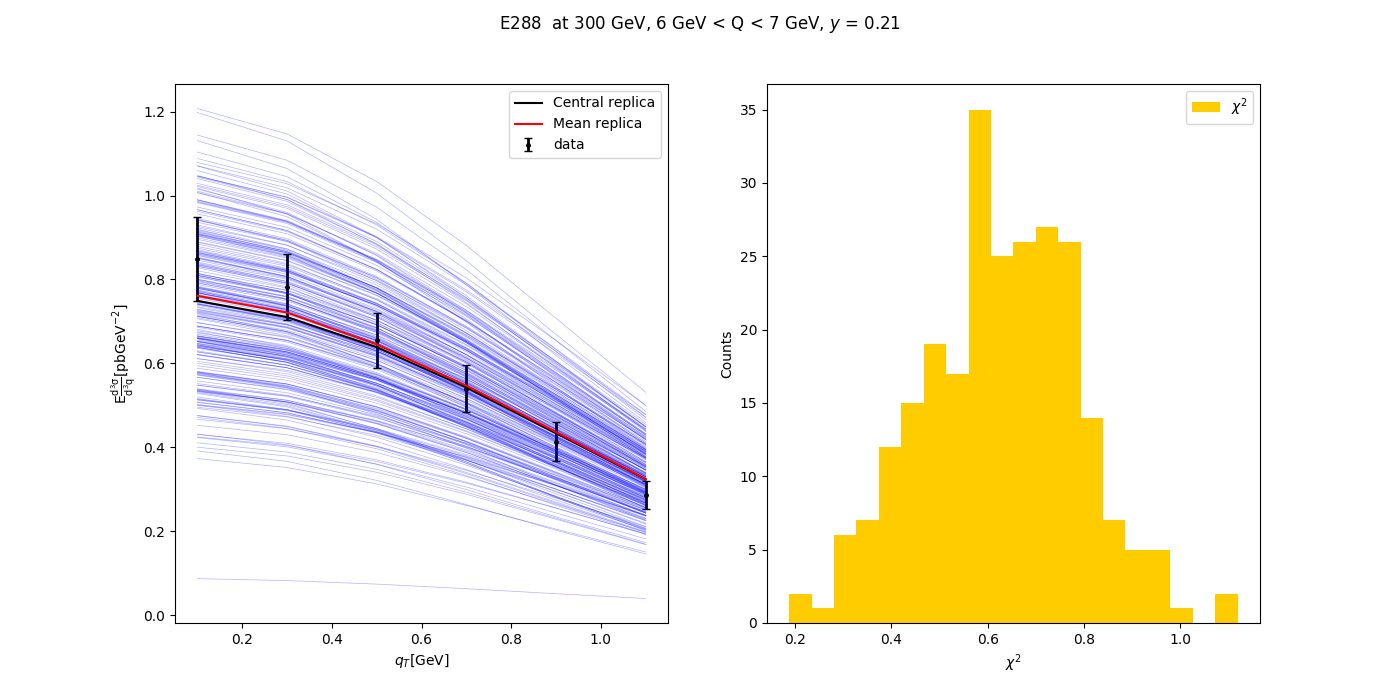
\includegraphics{pngplots/E288_300_Q_6_7.png}
\caption{E288\_300\_Q\_6\_7 data-theory comparison}
\end{figure}

\begin{figure}
\centering
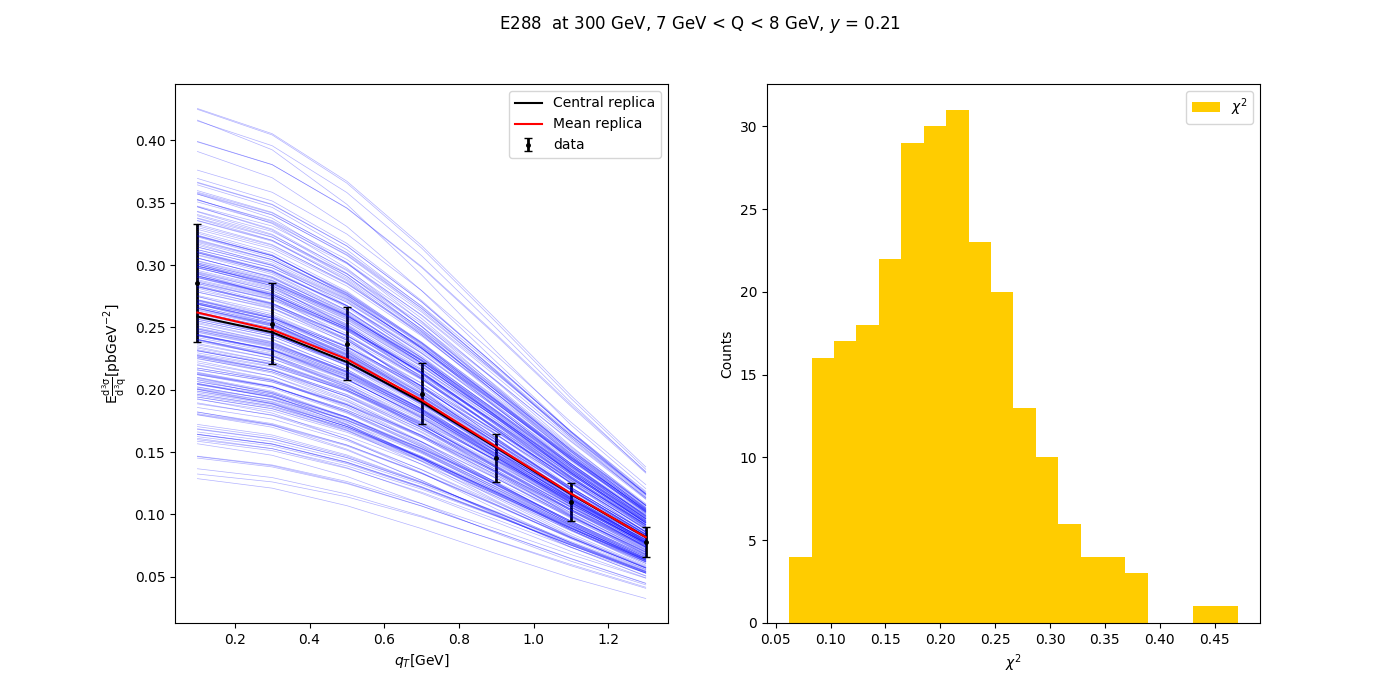
\includegraphics{pngplots/E288_300_Q_7_8.png}
\caption{E288\_300\_Q\_7\_8 data-theory comparison}
\end{figure}

\begin{figure}
\centering
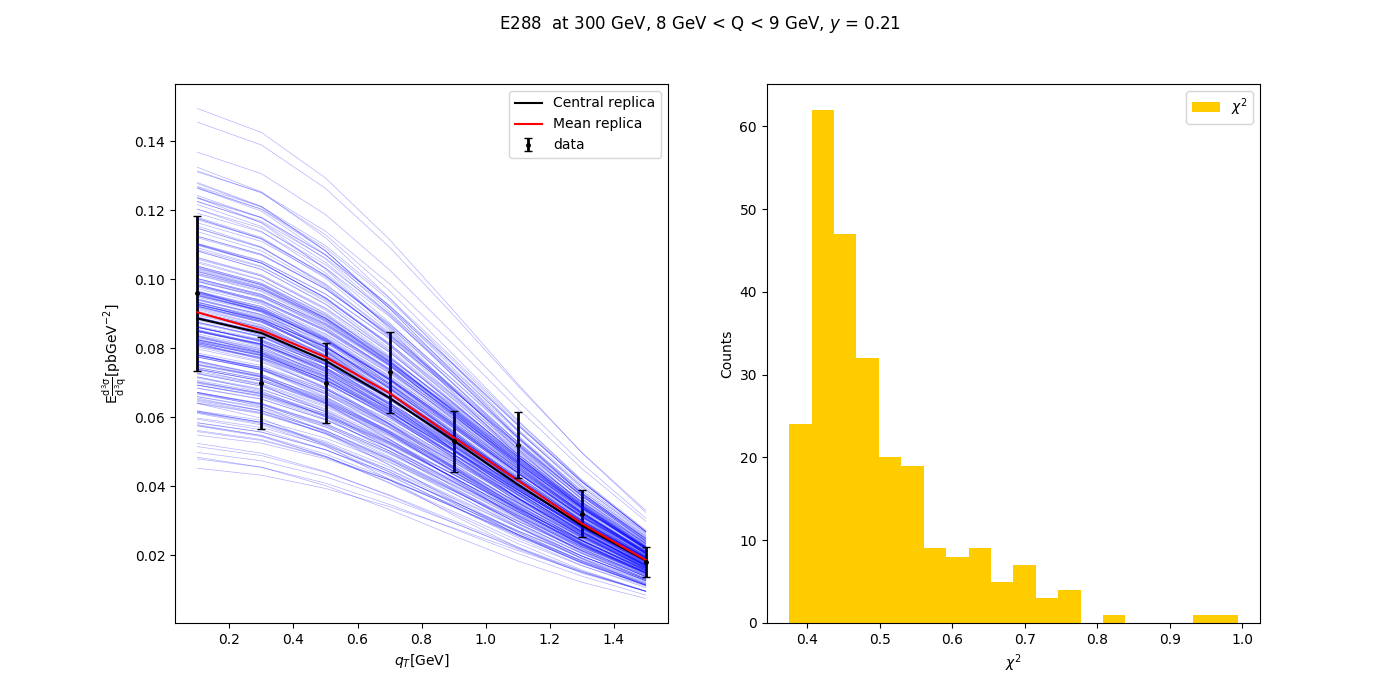
\includegraphics{pngplots/E288_300_Q_8_9.png}
\caption{E288\_300\_Q\_8\_9 data-theory comparison}
\end{figure}

\begin{figure}
\centering
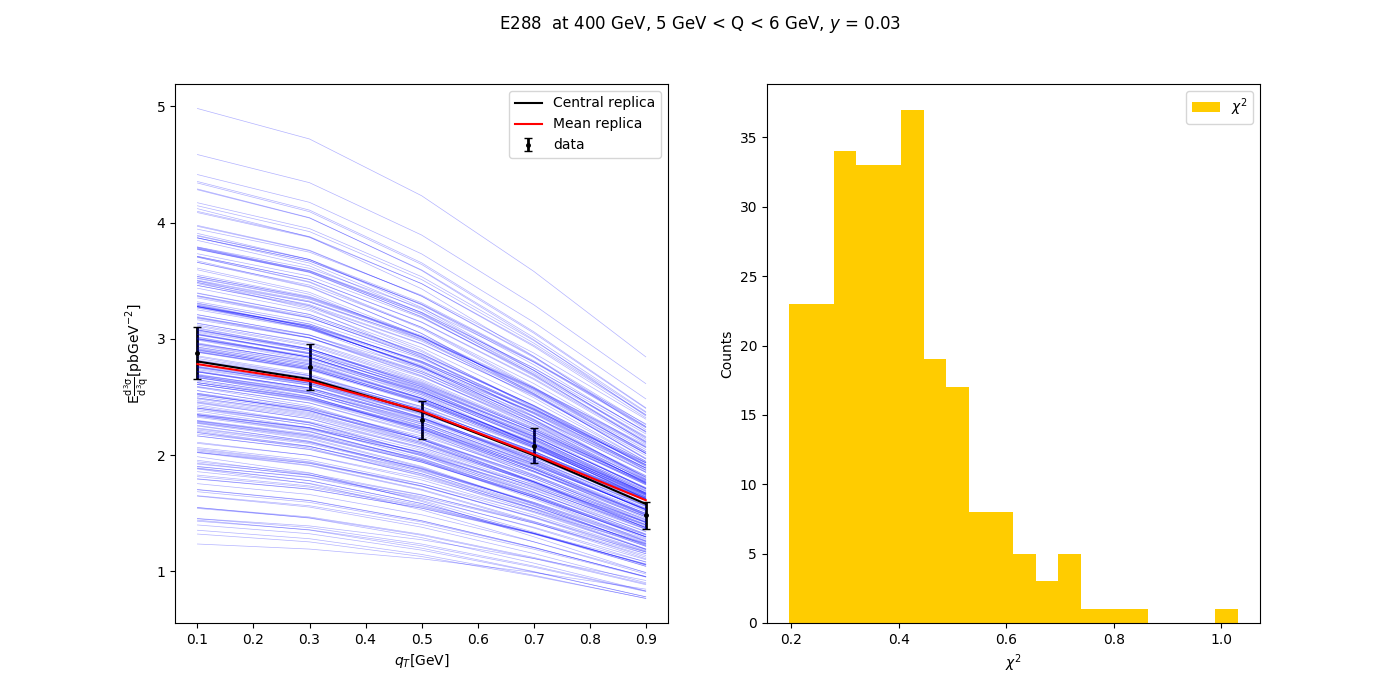
\includegraphics{pngplots/E288_400_Q_5_6.png}
\caption{E288\_400\_Q\_5\_6 data-theory comparison}
\end{figure}

\begin{figure}
\centering
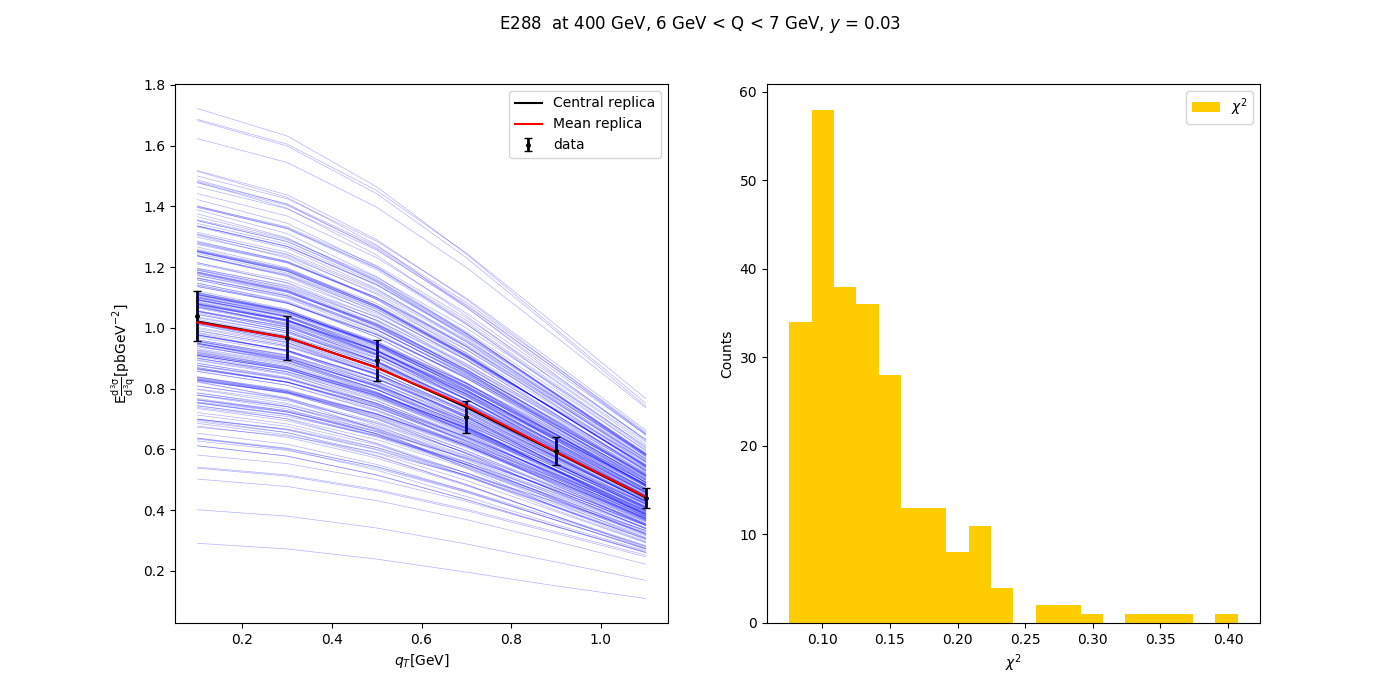
\includegraphics{pngplots/E288_400_Q_6_7.png}
\caption{E288\_400\_Q\_6\_7 data-theory comparison}
\end{figure}

\begin{figure}
\centering
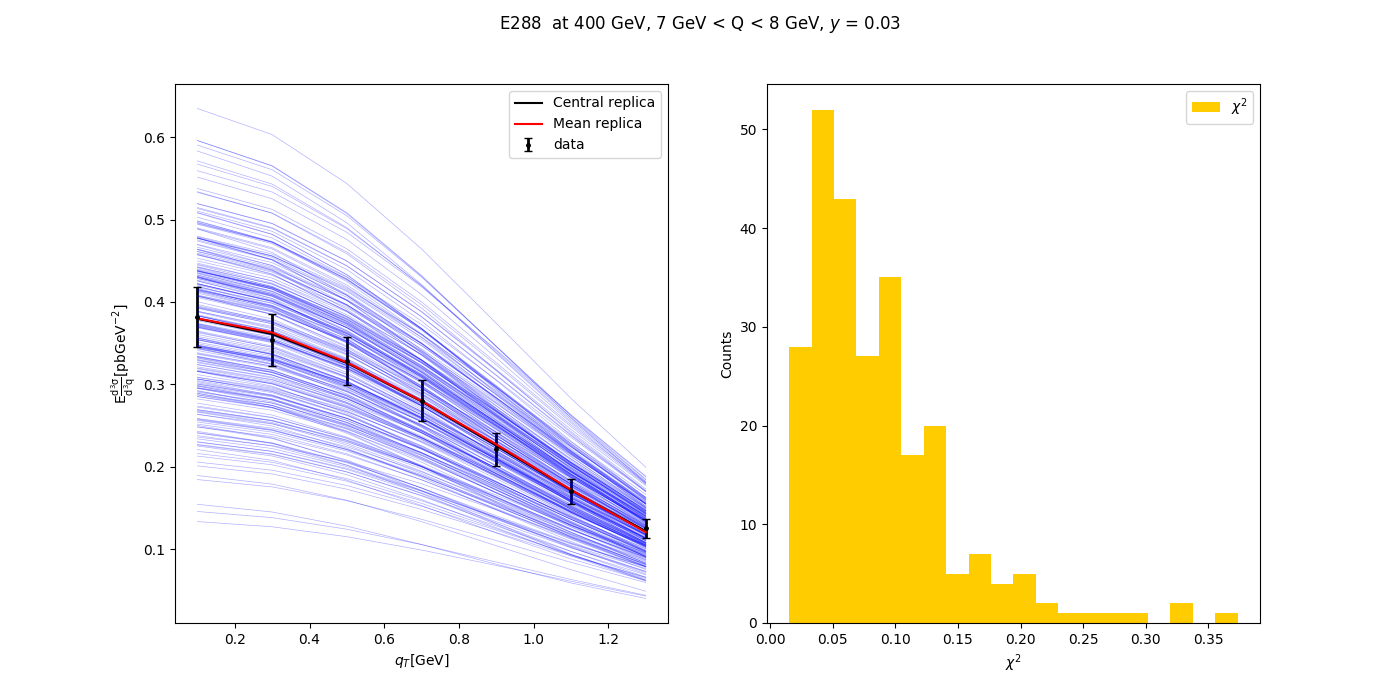
\includegraphics{pngplots/E288_400_Q_7_8.png}
\caption{E288\_400\_Q\_7\_8 data-theory comparison}
\end{figure}

\begin{figure}
\centering
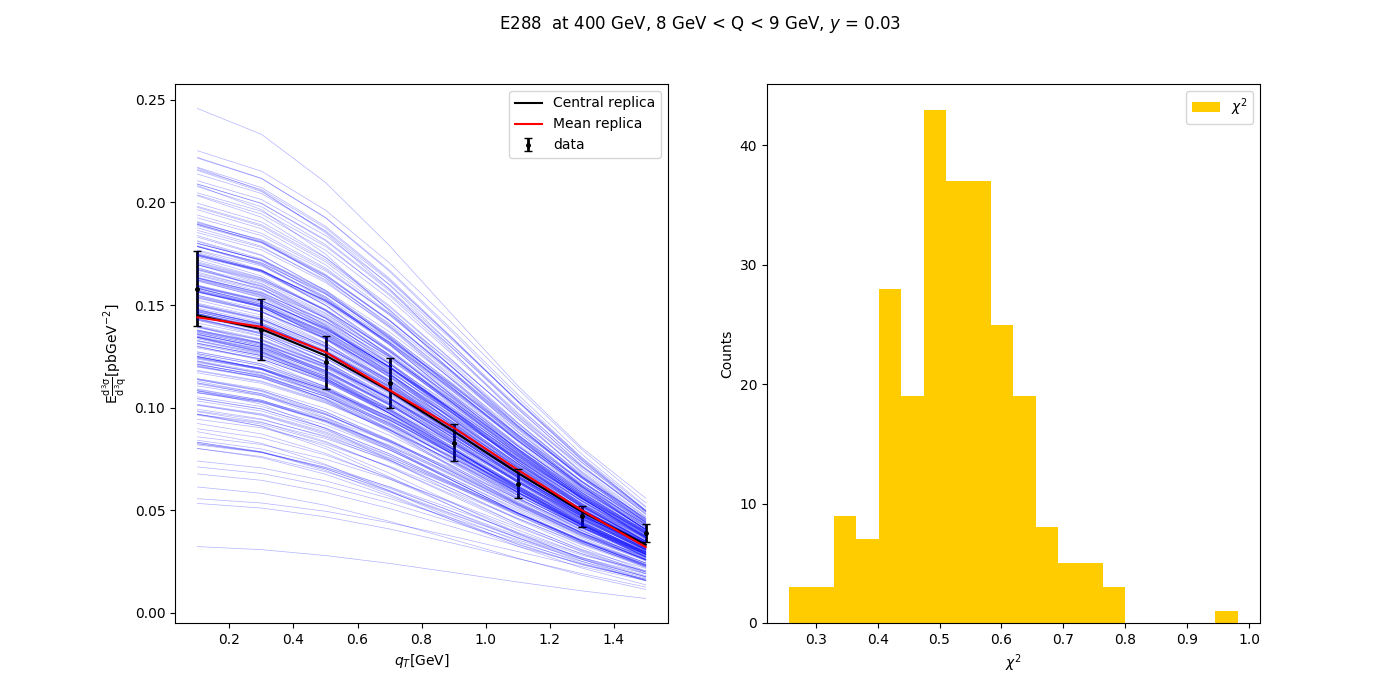
\includegraphics{pngplots/E288_400_Q_8_9.png}
\caption{E288\_400\_Q\_8\_9 data-theory comparison}
\end{figure}

\begin{figure}
\centering
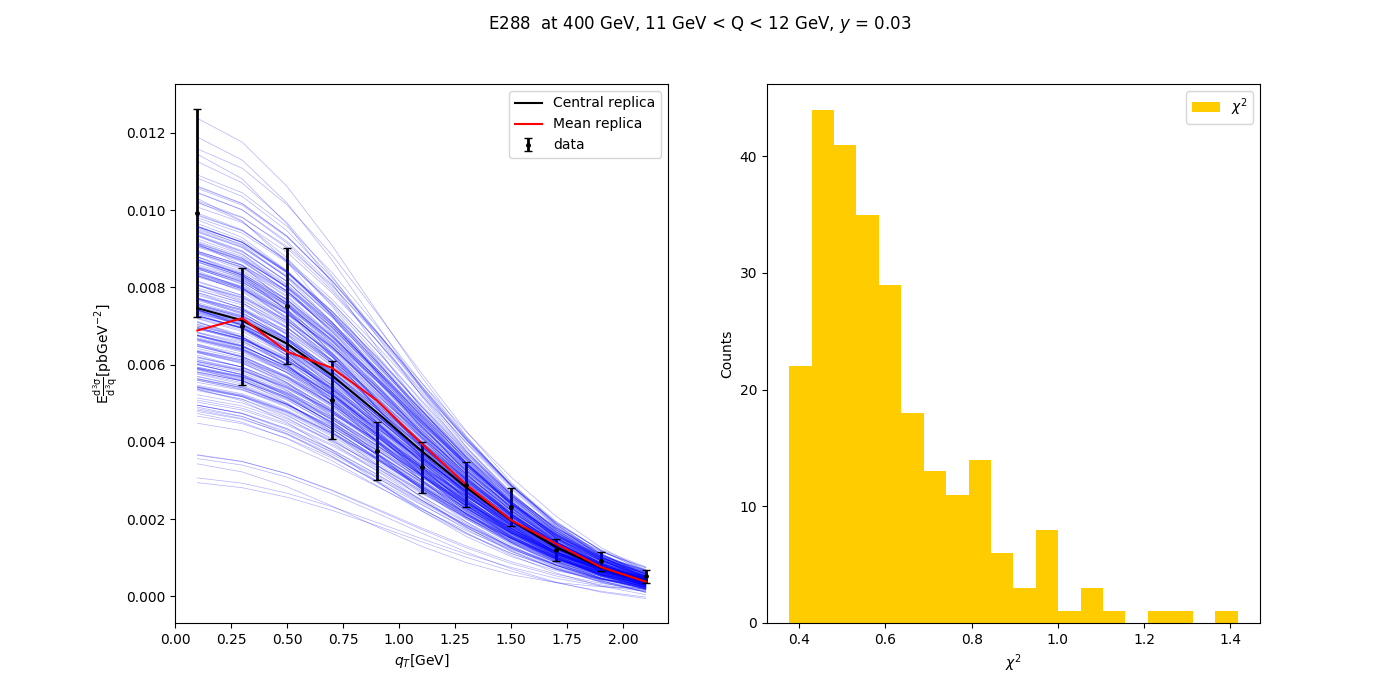
\includegraphics{pngplots/E288_400_Q_11_12.png}
\caption{E288\_400\_Q\_11\_12 data-theory comparison}
\end{figure}

\begin{figure}
\centering
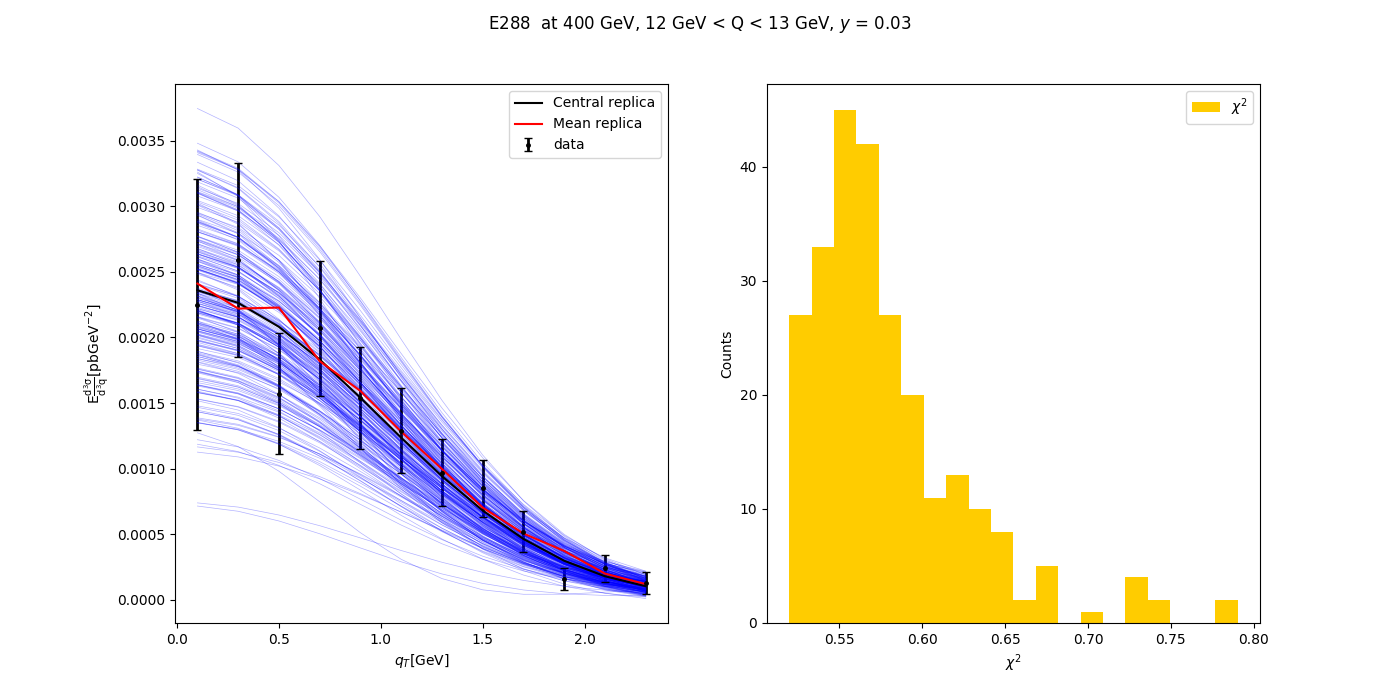
\includegraphics{pngplots/E288_400_Q_12_13.png}
\caption{E288\_400\_Q\_12\_13 data-theory comparison}
\end{figure}

\begin{figure}
\centering
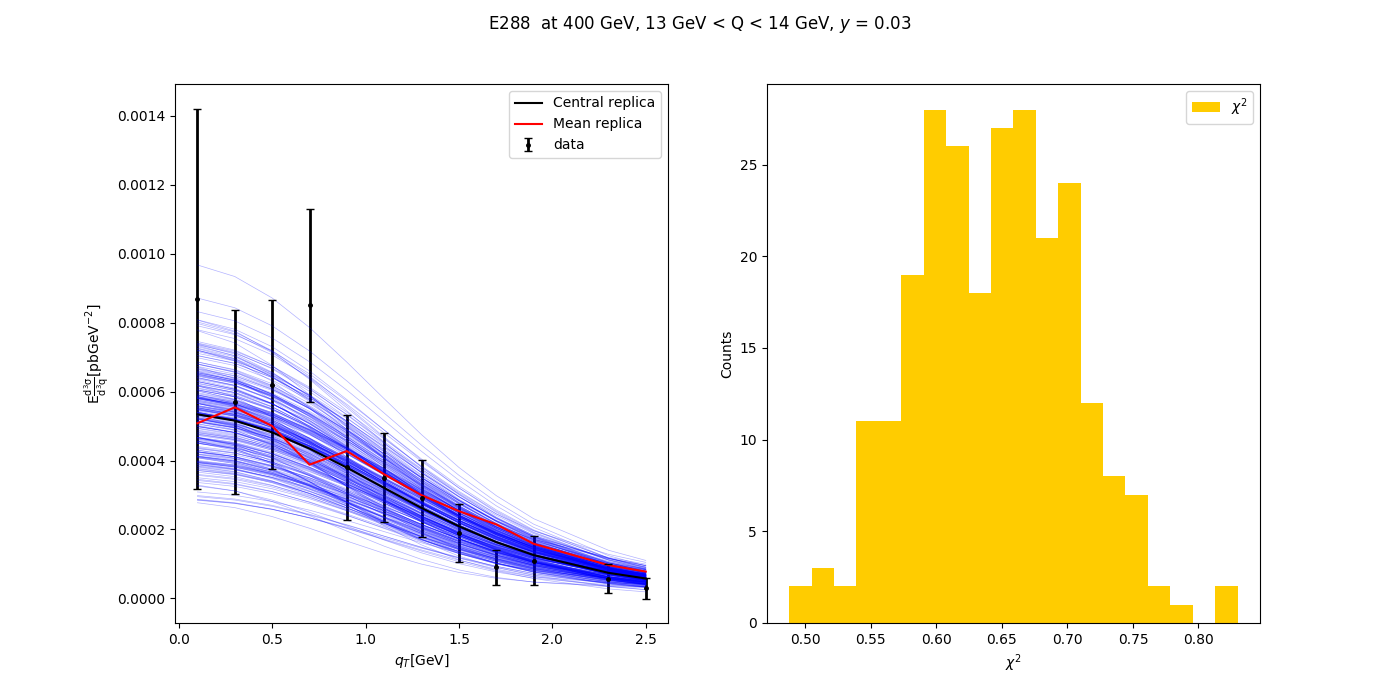
\includegraphics{pngplots/E288_400_Q_13_14.png}
\caption{E288\_400\_Q\_13\_14 data-theory comparison}
\end{figure}

\begin{figure}
\centering
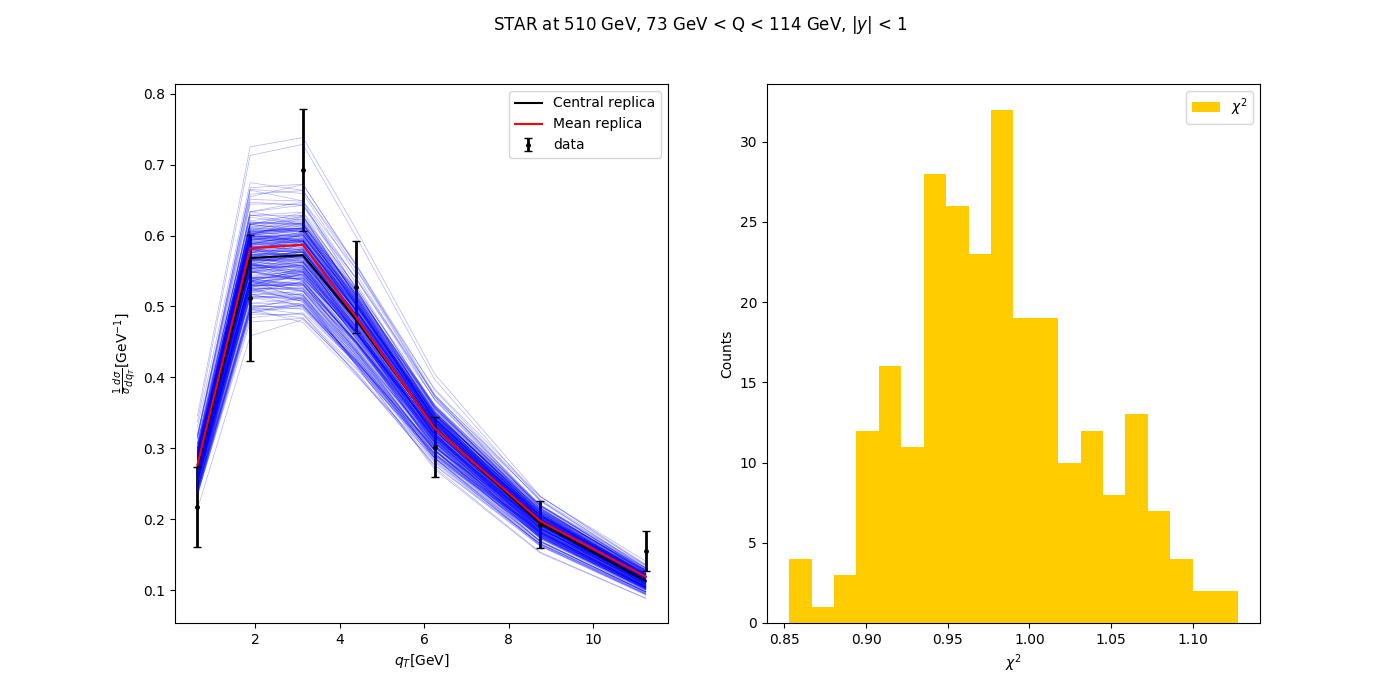
\includegraphics{pngplots/STAR_510.png}
\caption{STAR\_510 data-theory comparison}
\end{figure}

\begin{figure}
\centering
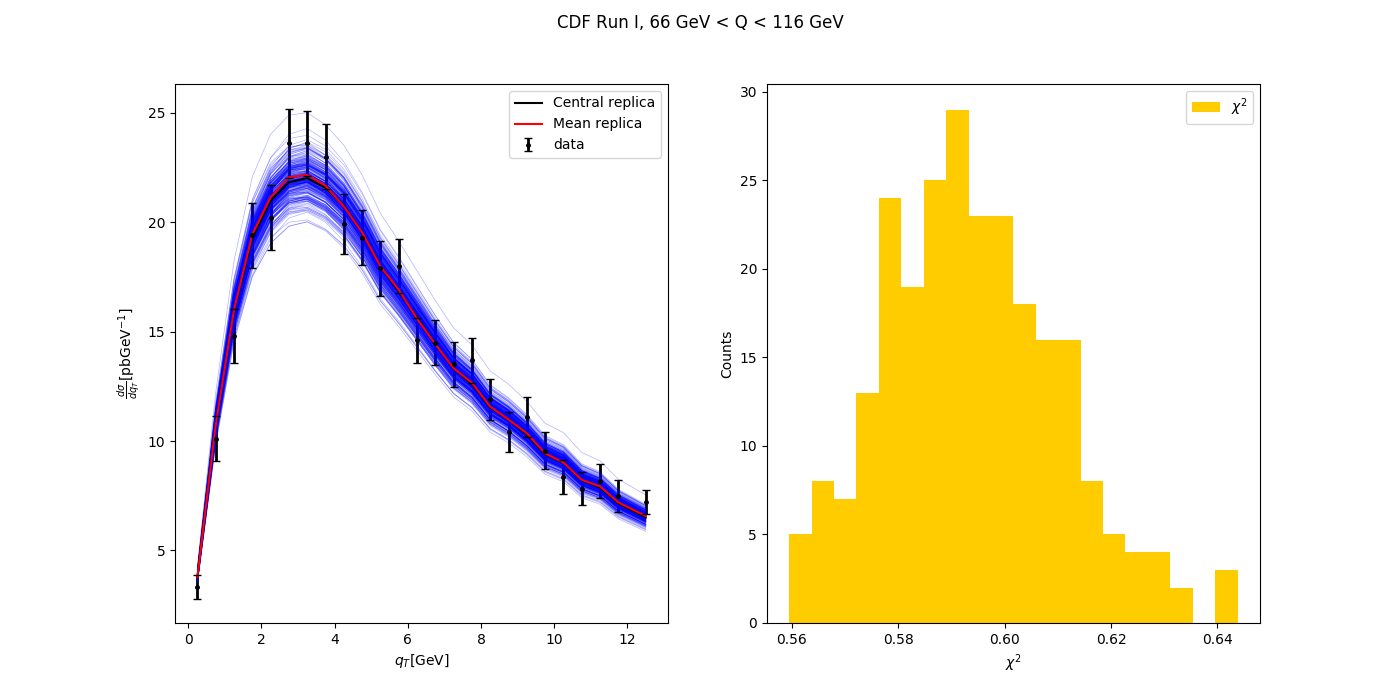
\includegraphics{pngplots/CDF_RunI.png}
\caption{CDF\_RunI data-theory comparison}
\end{figure}

\begin{figure}
\centering
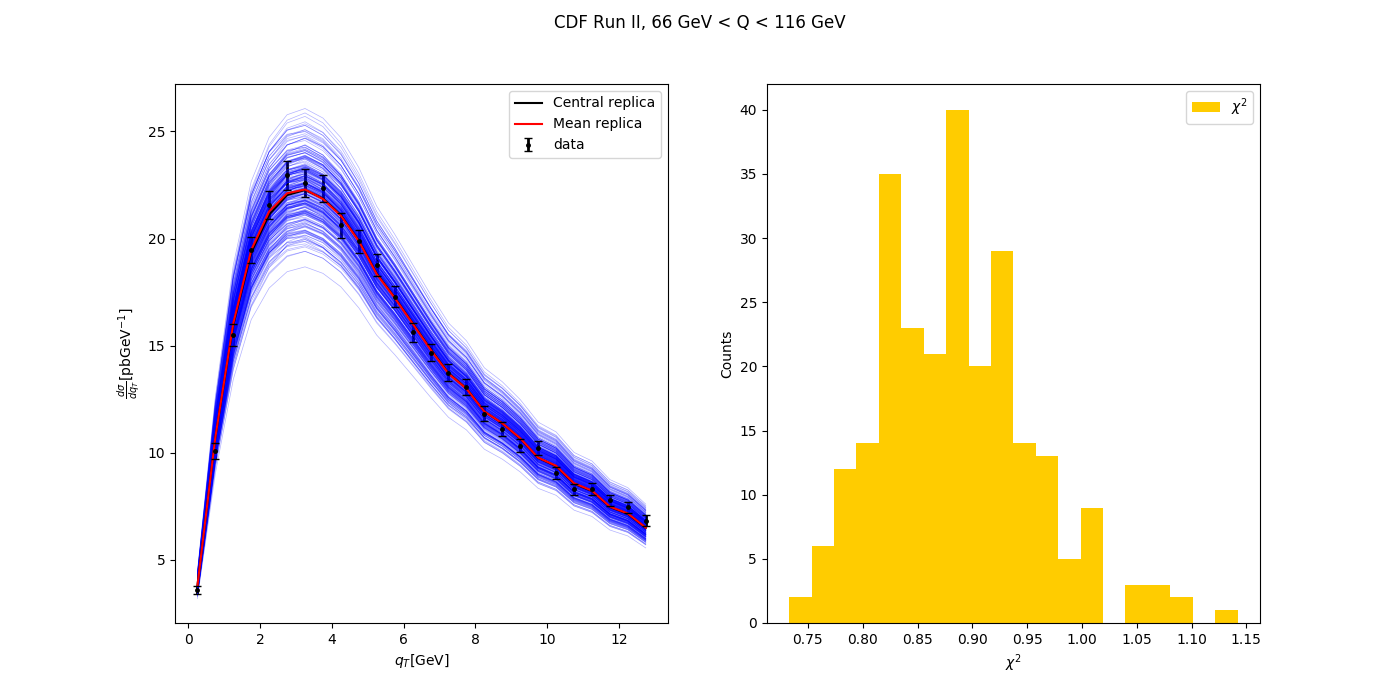
\includegraphics{pngplots/CDF_RunII.png}
\caption{CDF\_RunII data-theory comparison}
\end{figure}

\begin{figure}
\centering
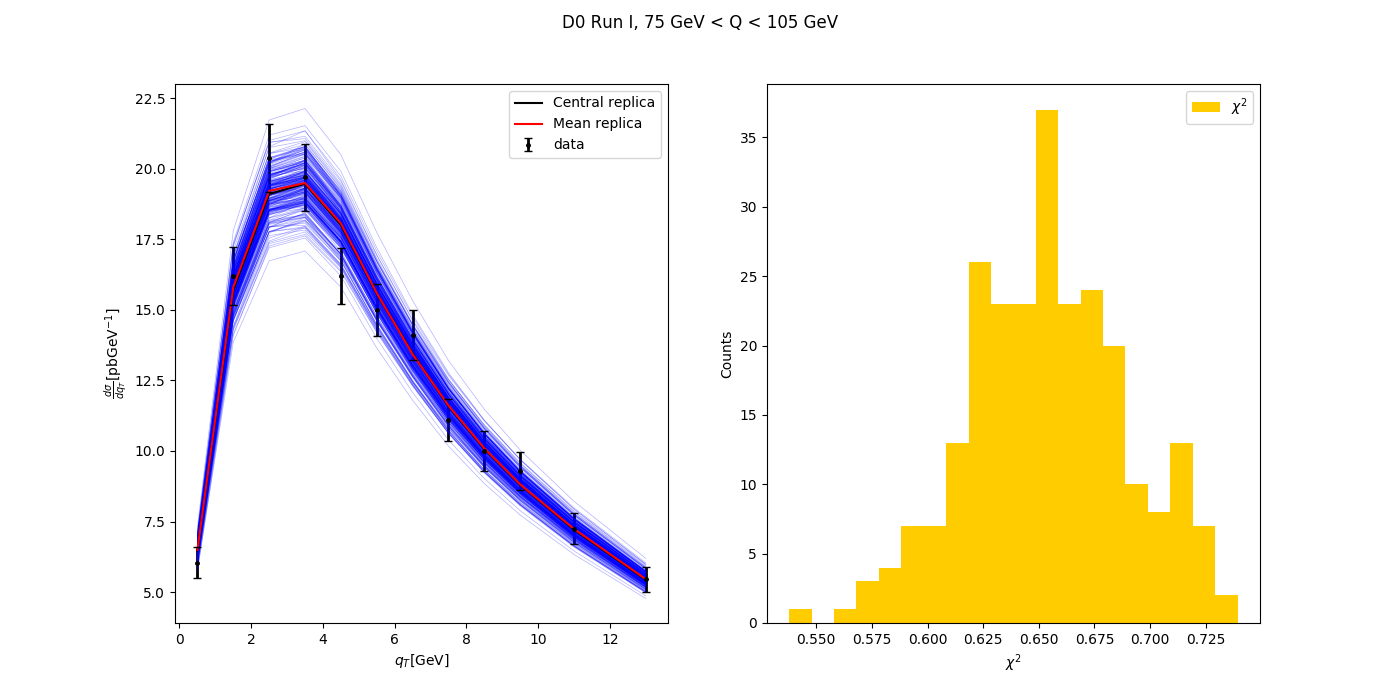
\includegraphics{pngplots/D0_RunI.png}
\caption{D0\_RunI data-theory comparison}
\end{figure}

\begin{figure}
\centering
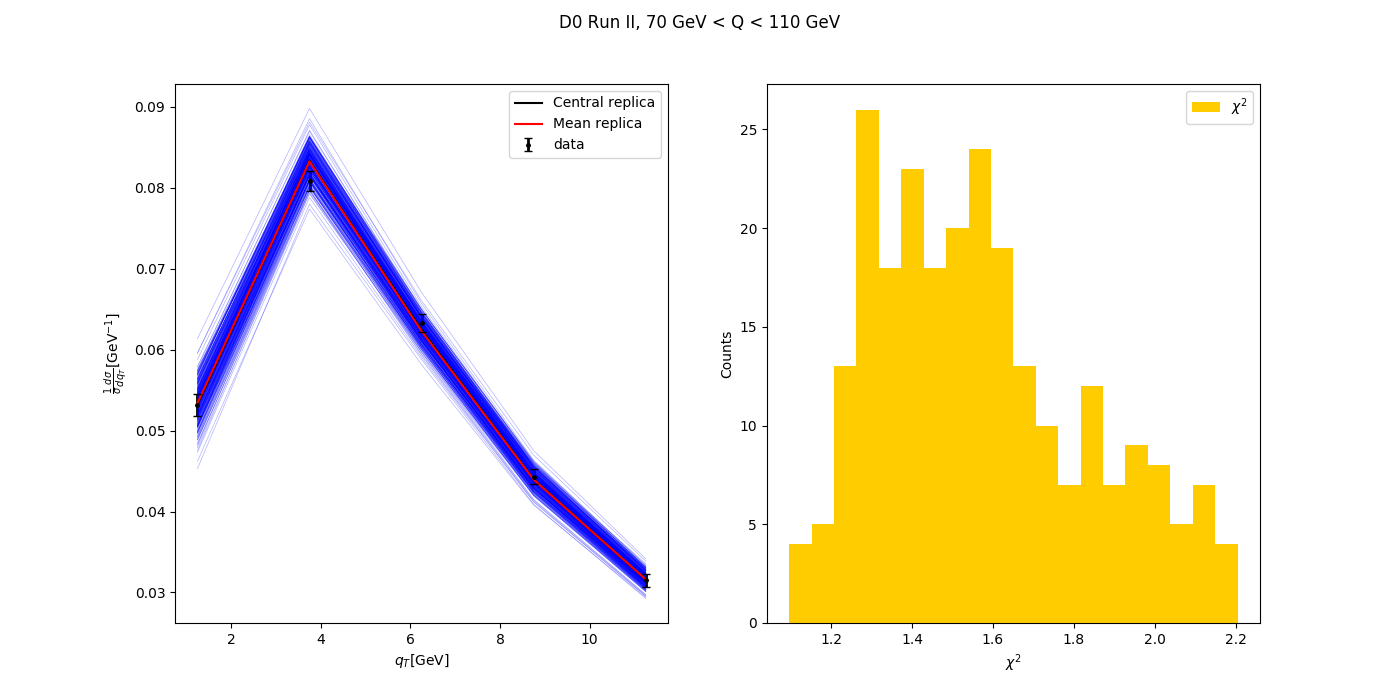
\includegraphics{pngplots/D0_RunII.png}
\caption{D0\_RunII data-theory comparison}
\end{figure}

\begin{figure}
\centering
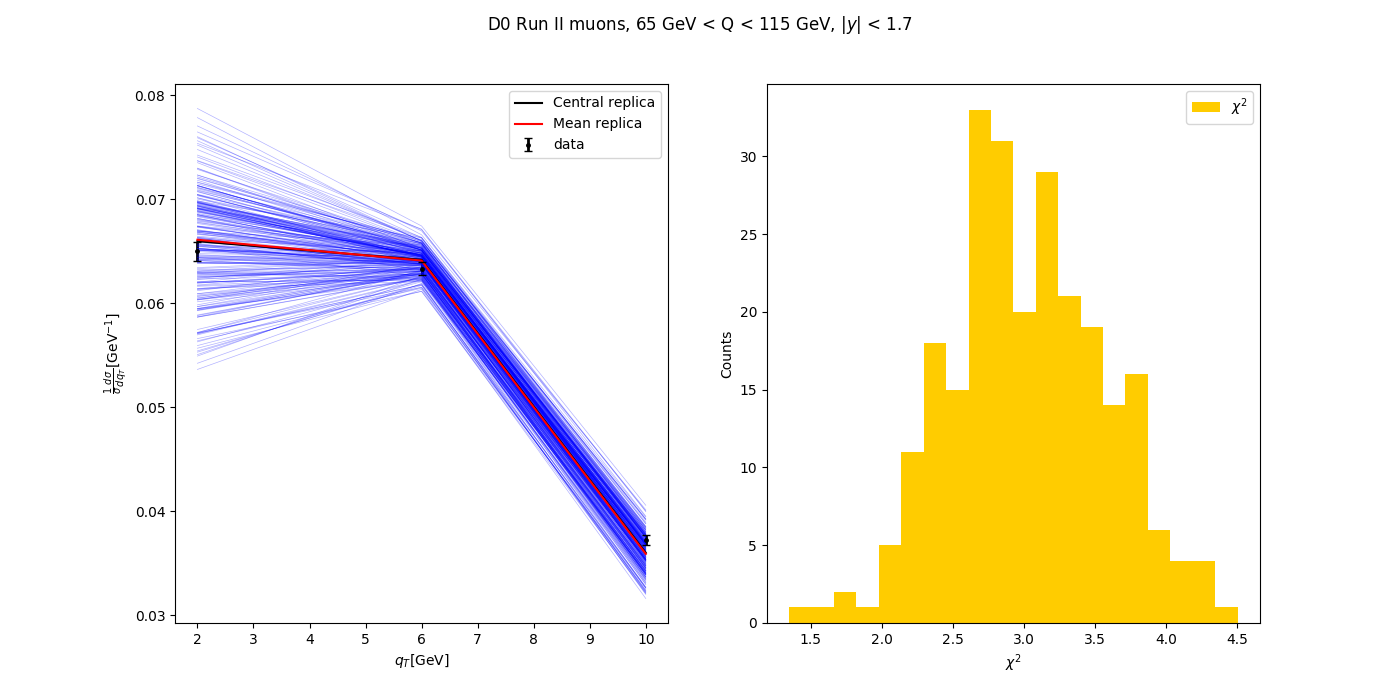
\includegraphics{pngplots/D0_RunIImu.png}
\caption{D0\_RunIImu data-theory comparison}
\end{figure}

\begin{figure}
\centering
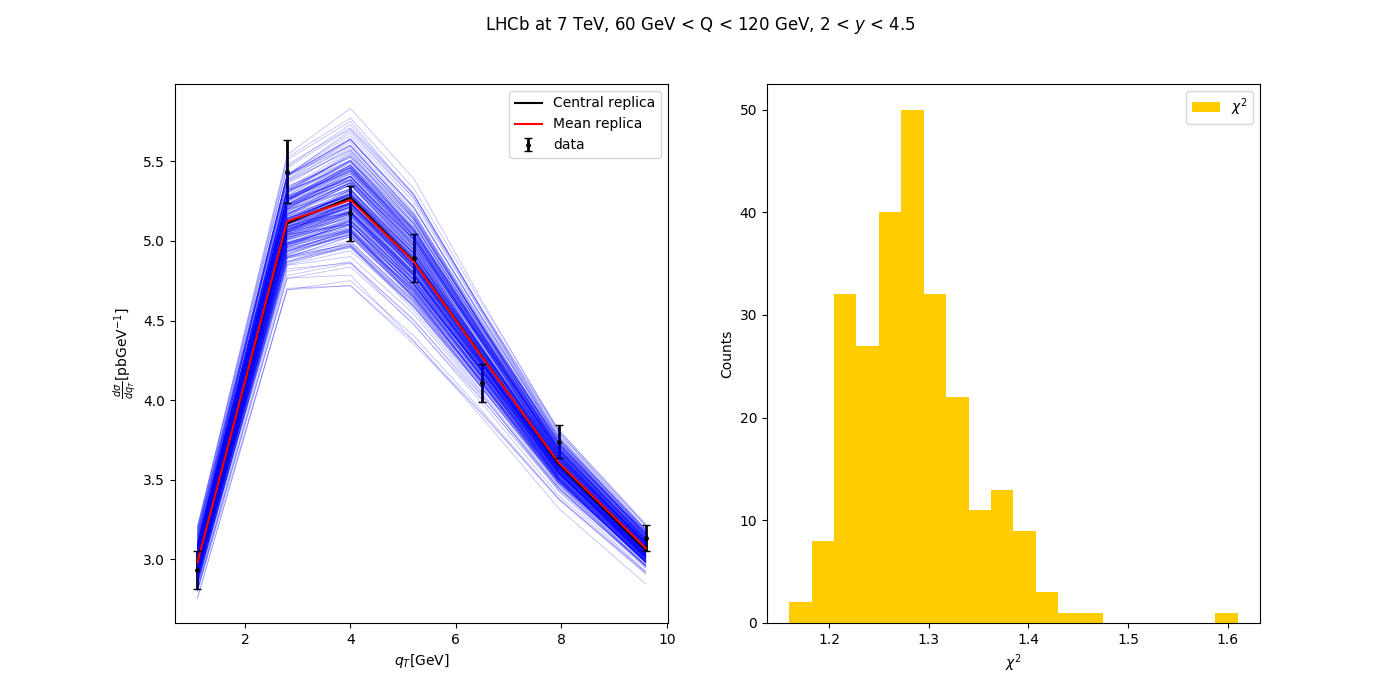
\includegraphics{pngplots/LHCb_7TeV.png}
\caption{LHCb\_7TeV data-theory comparison}
\end{figure}

\begin{figure}
\centering
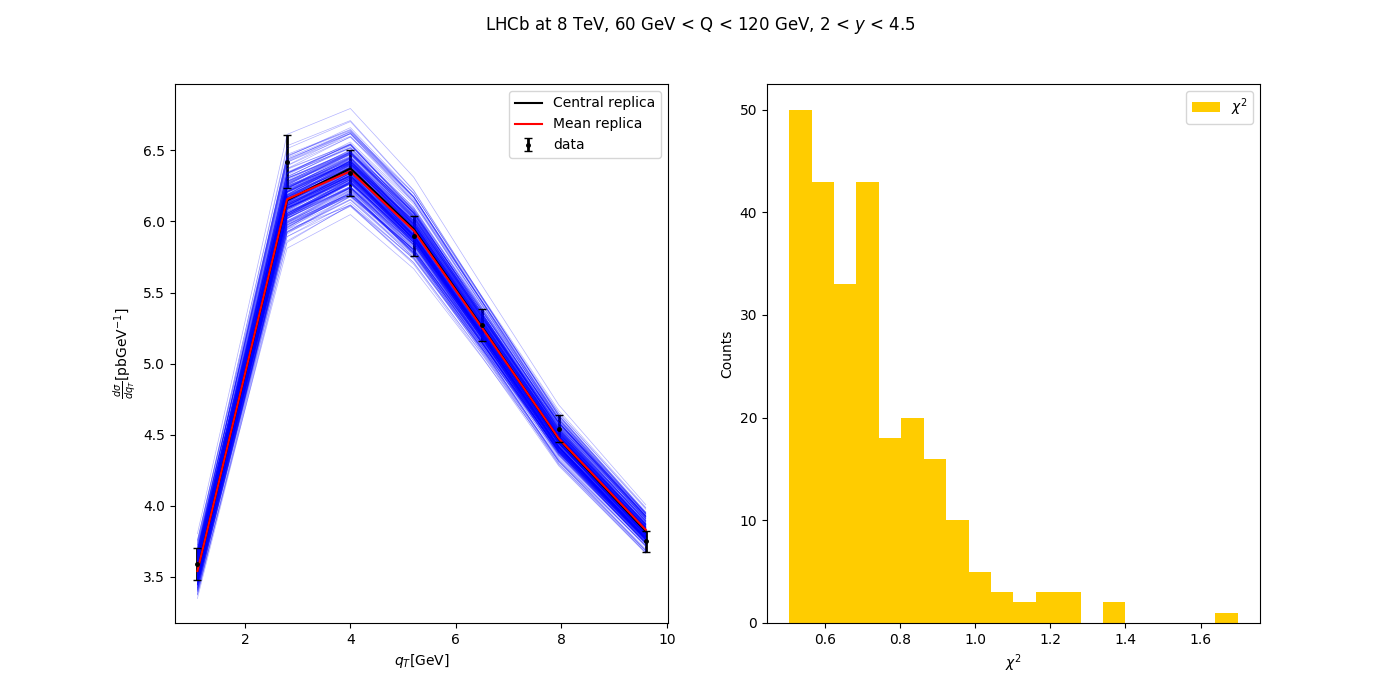
\includegraphics{pngplots/LHCb_8TeV.png}
\caption{LHCb\_8TeV data-theory comparison}
\end{figure}

\begin{figure}
\centering
\includegraphics{pngplots/LHCb_13TeV.png}
\caption{LHCb\_13TeV data-theory comparison}
\end{figure}

\begin{figure}
\centering
\includegraphics{pngplots/CMS_7TeV.png}
\caption{CMS\_7TeV data-theory comparison}
\end{figure}

\begin{figure}
\centering
\includegraphics{pngplots/CMS_8TeV.png}
\caption{CMS\_8TeV data-theory comparison}
\end{figure}

\begin{figure}
\centering
\includegraphics{pngplots/ATLAS_7TeV_y_0_1.png}
\caption{ATLAS\_7TeV\_y\_0\_1 data-theory comparison}
\end{figure}

\begin{figure}
\centering
\includegraphics{pngplots/ATLAS_7TeV_y_1_2.png}
\caption{ATLAS\_7TeV\_y\_1\_2 data-theory comparison}
\end{figure}

\begin{figure}
\centering
\includegraphics{pngplots/ATLAS_7TeV_y_2_2.4.png}
\caption{ATLAS\_7TeV\_y\_2\_2.4 data-theory comparison}
\end{figure}

\begin{figure}
\centering
\includegraphics{pngplots/ATLAS_8TeV_y_0_0.4.png}
\caption{ATLAS\_8TeV\_y\_0\_0.4 data-theory comparison}
\end{figure}

\begin{figure}
\centering
\includegraphics{pngplots/ATLAS_8TeV_y_0.4_0.8.png}
\caption{ATLAS\_8TeV\_y\_0.4\_0.8 data-theory comparison}
\end{figure}

\begin{figure}
\centering
\includegraphics{pngplots/ATLAS_8TeV_y_0.8_1.2.png}
\caption{ATLAS\_8TeV\_y\_0.8\_1.2 data-theory comparison}
\end{figure}

\begin{figure}
\centering
\includegraphics{pngplots/ATLAS_8TeV_y_1.2_1.6.png}
\caption{ATLAS\_8TeV\_y\_1.2\_1.6 data-theory comparison}
\end{figure}

\begin{figure}
\centering
\includegraphics{pngplots/ATLAS_8TeV_y_1.6_2.png}
\caption{ATLAS\_8TeV\_y\_1.6\_2 data-theory comparison}
\end{figure}

\begin{figure}
\centering
\includegraphics{pngplots/ATLAS_8TeV_y_2_2.4.png}
\caption{ATLAS\_8TeV\_y\_2\_2.4 data-theory comparison}
\end{figure}

\begin{figure}
\centering
\includegraphics{pngplots/ATLAS_8TeV_Q_46_66.png}
\caption{ATLAS\_8TeV\_Q\_46\_66 data-theory comparison}
\end{figure}

\begin{figure}
\centering
\includegraphics{pngplots/ATLAS_8TeV_Q_116_150.png}
\caption{ATLAS\_8TeV\_Q\_116\_150 data-theory comparison}
\end{figure}

\end{document}
